%%%% fatec-article.tex, 2024/03/10

%% Classe de documento
\documentclass[
  a4paper,%% Tamanho de papel: a4paper, letterpaper (^), etc.
  12pt,%% Tamanho de fonte: 10pt (^), 11pt, 12pt, etc.
  english,%% Idioma secundário (penúltimo) (>)
  brazilian,%% Idioma primário (último) (>)
]{article}

\usepackage{pdflscape}
\usepackage[]{fatec-article}
\Author{1}{Name={Queiroz.I\\ Kusaka.J \\ Abrahão.M\\ Rodrigues.T\\ Roder.V}}

\Author{2}{Name={\{ isabele.queiroz@fatec.sp.gov.br \}\\ \{ joao.kusaka@fatec.sp.gov.br \} \\ \{ matheus.abrahao@fatec.sp.gov.br\} \\ \{ tiago.rodrigues39@fatec.sp.gov.br \} \\ \{victor.roder@fatec.sp.gov.br \}}}

\Keyword{1}{Carcinicultura}{Shrimp Farming}
\Keyword{2}{Monitoramento}{Monitoring}
\Keyword{3}{Sustentável}{Sustainability}

\begin{Abstract}[brazilian]
  No cenário mundial, a carcinicultura é uma atividade de grande importância econômica e ambiental, com o Brasil se destacando como um dos principais produtores de camarão, especialmente no Nordeste. No entanto, a criação de camarões enfrenta desafios significativos, como a má gestão dos tanques, que pode causar poluição da água, proliferação de doenças e baixa qualidade dos camarões. Para superar esses desafios e se alinhar com os Objetivos de Desenvolvimento Sustentável (ODS) 12 e 14, propõe-se um sistema de monitoramento 24 horas para cativeiros de camarões, utilizando arduínos e Inteligência Artificial (IA). Este sistema monitora parâmetros essenciais da água, como temperatura, pH e níveis de amônia, além de automatizar a alimentação dos camarões e armazenar dados para análises futuras. A plataforma web permitirá que os usuários visualizem dados de cada cativeiro, gerenciem informações e automatizem a alimentação, contribuindo para uma produção mais sustentável e eficiente. Com os resultados apresentados, este sistema tem como promessa se tornar um sistema de alta qualidade para os carcinicultores.

\end{Abstract}

\begin{Abstract}[english]
In the global scenario, shrimp farming stands out as an economically and environmentally significant activity, with Brazil emerging as one of the major producers, particularly in the Northeast region. However, shrimp cultivation encounters significant challenges, such as poor tank management leading to water pollution, disease outbreaks, and compromised shrimp quality. To address these challenges and align with Sustainable Development Goals (SDGs) 12 and 14, a 24-hour monitoring system for shrimp farms is proposed, leveraging Arduinos and Artificial Intelligence (AI). This system monitors crucial water parameters like temperature, pH, and ammonia levels, automates shrimp feeding, and stores data for future analysis. The associated web platform enables users to visualize farm data, manage information, and automate feeding, thereby fostering more sustainable and efficient production practices. With the presented results, this system holds the promise of becoming a high-quality solution for shrimp farmers.
\end{Abstract}


\makeindex


\addbibresource{fatec-article.bib}

\begin{document}

\section*{Introdução}%
\label{sect:intro}
No ano de 1945, após a Segunda Guerra Mundial, foi fundada a Organização das Nações Unidas (ONU) com o intuito de garantir a paz e a segurança para o planeta por meio da colaboração dos países. Atualmente, conta com o total de 193 estados que compõem a Assembleia Geral. No ano de 2015, os 193 líderes mundiais se comprometeram com os Objetivos de Desenvolvimento Sustentável (ODS) \cite{ODS12}na Agenda 2030, um plano de desenvolvimento para acabar com a pobreza, cuidar do meio ambiente e do clima, e garantir que as pessoas, em qualquer região do planeta, desfrutem da paz e prosperidade. 

Entre os Objetivos de Desenvolvimento Sustentável, destacam-se os ODS 12 (Produção e Consumo Sustentáveis) e ODS 14 (Oceanos, Mares e Recursos Marinhos). A ODS 12 diz respeito à garantia da qualidade de produção e consumo de alimentos, visando à saúde humana e à diminuição dos impactos ambientais que podem ser causados. A ODS 14, por sua vez, busca a proteção de animais e ecossistemas marinhos, com o intuito de prevenir problemas como poluição, doenças e destruição de habitats naturais.

A carcinicultura, técnica de criação de camarões em viveiros, é amplamente praticada no Brasil. De acordo com \cite{Rocha2023}, a produção de camarão vem crescendo a uma taxa de 4,97\% nos últimos 7 anos. O Equador é atualmente o maior produtor e exportador mundial, com uma produção aproximada de 1.430.000 toneladas e exportação de cerca de 1.215.000 toneladas apenas em 2023, seguido por China, Índia, Vietnã, Indonésia, Tailândia e Brasil \cite{Rocha2024}. No Brasil, o camarão representa a segunda maior fonte de valor entre as espécies cultivadas. O Ceará se destaca como o maior produtor, com 43.778.493 toneladas produzidas em 2022, e o Nordeste responde por cerca de 99\% da produção total de camarão, que atingiu 92.438,960 toneladas no mesmo ano \cite{Ximenes2023}.

O Vale do Ribeira, localizado no sul do estado de São Paulo, tem como uma de suas principais atividades econômicas a criação de camarões. A região, com seu clima favorável e presença de rios, estuários e manguezais, oferece um ambiente adequado para a carcinicultura. A produção local é impulsionada tanto por turistas que adquirem camarões diretamente dos produtores quanto por restaurantes e outras fazendas.

Os carídeos dulcícolas (crustáceos de água doce), representados principalmente pelas famílias Palaemonidae e Atyidae, também são encontrados na região do Vale do Ribeira. A família Palaemonidae inclui cerca de 980 espécies e está dividida em duas subfamílias: Pontoniinae e Palaemoninae. Esta última possui 18 gêneros, dos quais Palaemon, Palaemonetes e Macrobrachius são os mais representativos. A família Atyidae é composta por 469 espécies distribuídas em 42 gêneros \cite{bertini2021}.

Entretanto, a criação de camarões enfrenta desafios significativos, como a falta de cuidado com os tanques e a infraestrutura, o que pode resultar em poluição da água, acúmulo de resíduos e proliferação de doenças entre os camarões. A má gestão dos tanques afeta negativamente a qualidade e a produtividade da criação, prejudicando tanto o consumidor quanto o produtor.

Para enfrentar esses desafios e melhorar a qualidade da produção, torna-se necessário investir em tecnologias avançadas. Uma solução promissora é a implementação de um sistema de monitoramento por meio de **Inteligência Artificial (IA)**. A **IA** é um campo de estudo que visa o desenvolvimento de sistemas capazes de realizar tarefas que exigem inteligência humana. Por meio de algoritmos e cálculos matemáticos, a **IA** pode aprender com base em dados, reconhecendo padrões e tomando decisões de forma autônoma.

Neste contexto, o projeto proposto visa à criação de um sistema de monitoramento automatizado utilizando IA e sistemas embarcados. Esse sistema será responsável por monitorar as condições dos tanques de criação, incluindo parâmetros como temperatura, pH, oxigênio e níveis de amônia. O objetivo não é apenas a coleta de dados, mas também a análise preditiva dessas informações, permitindo o ajuste automático de condições para otimizar a saúde dos camarões e prevenir problemas antes que se tornem críticos. Isso resultaria em uma melhoria significativa na gestão dos viveiros, reduzindo o risco de doenças e aumentando a produtividade de forma sustentável.


\section*{OBJETIVO} \label{sect:obj}

Este sistema de monitoramento tem como meta auxiliar os produtores para criarem camarões de boa qualidade e manter o controle do cativeiro. Dentre os objetivos estão: 	 

\begin{enumerate}

\item Criar um ambiente de monitoramento remoto por 24 horas para total cuidado dos cativeiros. 

\item Manter o controle de pH da água alertando para caso ocorra algum tipo de mudança no pH, assim criando um ambiente de boa qualidade para os camarões impedindo que fiquem com problemas de desenvolvimento. 

\item Monitorar a temperatura da água do cativeiro para manter o ambiente estável para o camarão. 

\item Monitorar os níveis de amônia na água para a prevenção de condições tóxicas para os camarões. 

\item Armazenar dados dos cativeiros e dos camarões para futuras comparações de qualidade. 

\item Controle de horário e automatização da alimentação dos camarões para boa nutrição.

\end{enumerate}

\section*{ESTADO DA ARTE} \label{sect:estadoarte}

A realização de um sistema de monitoramento para cuidado dos camarões é de grande importância, ajuda tanto o produtor a vender um produto de qualidade, tanto o consumidor que irá consumir algo de qualidade sem prejudicar a sua saúde. Por conta desta importância, é de se imaginar que já possam existir sistemas parecidos. Dentre os projetos já existentes, há de se destacar determinados artigos.

O trabalho\cite{dantas2020} é proposto um sistema de telemonitoramento e automação baseado em rede LoRaWAN. O artigo descreve o desenvolvimento de um sistema de monitoramento de temperatura e pH e automação de viveiros de camarão utilizando tecnologia LoRa. A plataforma visa auxiliar carcinicultores, engenheiros de pesca e colaboradores das fazendas de criação no cultivo de camarões. A comunicação entre os nós sensores e o gateway é realizada via protocolo LoRaWAN, permitindo a transferência de dados para a nuvem através de um broker MQTT.

Os resultados registraram as médias de cada setor trabalhado. A temperatura obteve a média de 0 a 80°C. O pH apresentou uma média entre 6,64 e 7,5.

\cite{Uddin2020} diz a respeito de um sistema de monitoramento de fazendas de camarão de água doce baseado em IoT. O sistema tem a proposta de monitorar a qualidade da água como temperatura, pH, salinidade, oxigênio dissolvido e turbidez e verificar o peso, tamanho e porcentagem de sobrevivência por meio de IoT. Isso porque envolve a coleta de dados de sensores em tempo real, armazenamento desses dados na nuvem e disponibilização de visualização e análise desses dados por meio de uma aplicação web. A camada física do sistema utiliza sensores para coletar dados e uma placa arduíno para processamento e transmissão desses dados para a nuvem.

Os resultados indicaram que o sistema funciona de maneira eficiente, com bons níveis de precisão, a temperatura obteve 98,\%, nível de pH obteve 98,24\%, salinidade obteve 94,12\%, oxigênio obteve 95,46\%, turbidez obteve 93,55\%. Os camarões atingiram tamanhos entre 9 e 12 cm, peso varia entre 10 e 20g e a taxa de sobrevivência obteve 90\%. 

\cite{Zainuddin2019} apresenta um sistema de monitoramento da qualidade da água para cultivo de camarão Vannamae baseado em rede de sensores sem fios. O sistema proposto consiste em sensores para monitorar temperatura, pH e turbidez da água, integrados a microcontroladores e dispositivos de comunicação sem fio em conjunto de IoT. Os resultados do estudo incluem aspectos de hardware e software, destacando a produção de unidades transmissoras e receptores, bem como os testes de calibração dos sensores.

Os resultados indicam que o sistema pode funcionar bem, com altos níveis de precisão nos sensores de temperatura com 97,76\%, pH com 98,85\% e turbidez com 99,73\%.

Em geral, os três projetos se assemelham em diversos fatores, como o monitoramento de temperatura e pH da água, a criação de um sistema de monitoramento e o uso de IoT. Um dos três artigos citados trabalha acerca do peso e tamanho do camarão. 

Em comparação com os artigos anteriores, pode-se notar a diferença encontrada em nosso projeto. Ao invés de apenas o uso de IoT, contará com o uso de IA para auxiliar em tarefas como coleta de dados pelo hardware, criação de relatórios a partir das informações coletadas, analisar os dados para alertas sobre possíveis riscos caso ocorra uma mudança tanto nas condições dos tanques tanto na alimentação. Irá controlar a alimentação dos camarões para uma alimentação saudável com comestíveis apropriados para seu consumo, sua alimentação irá se basear em estimativas de crescimento e sobrevivência dos camarões nos cativeiros, caso não sejam controlados adequadamente, geram perdas econômicas e problemas nos cativeiros. Irá monitorar os níveis de amônia e irá realizar comparações com outros cativeiros.

\section*{METODOLOGIA} \label{sect:metodologia}

Neste projeto, foram utilizados uma série de ferramentas e técnicas para auxiliar no desenvolvimento do web. Estas abordagens incluem o uso do Figma, uma plataforma colaborativa para design de interfaces e protótipos pertencente à empresa Figma, INC, do Modelo de Negócios Canvas, uma ferramenta de planejamento estratégico, do DER (Diagrama de Entidade e Relacionamento) e o Oracle Apex, uma plataforma de desenvolvimento de aplicações Low Code.

O Figma será empregado como uma plataforma colaborativa de design para desenvolver os protótipos da interface do usuário do aplicativo. Isso possibilitará que a equipe de design trabalhe de forma conjunta, recebendo feedback instantâneo. Dessa forma, asseguraremos que a interface do usuário seja intuitiva e visualmente atrativa \cite{lopes2023}. 

O Modelo de Negócios Canvas é uma representação detalhada e abrangente da operação, receita e valor que uma empresa proporciona aos seus clientes. Ele visa auxiliar no desenvolvimento da percepção para entendimento da vida em sociedade o papel que lhes é atribuído. No caso específico, o canvas será utilizado para criar uma representação visual do projeto dentro do mercado gastronômico de camarões. Isso ajudará a equipe a identificar parceiros-chave, recursos-chave, atividades-chave e fontes de receita. O objetivo é assegurar que o projeto esteja alinhado tanto com os objetivos científicos quanto com os de negócios \cite{biava2017}. 

A plataforma de criação Apex, será capaz de capacitar os desenvolvedores a criar facilmente aplicativos com funcionalidades, desempenho e experiência. Sem muitas complexidades no desenvolvimento e implantação de aplicativos empresariais. Fornecendo uma interface rica e intuitiva, o resultado é uma aplicação Low Code mais rápida, mais leve e com custos menores. 

Utilizaremos a plataforma para gerenciar informações de registros como dados de usuários, localização de cativeiros, restrições necessárias 

Em comparação com aplicativos de camada intermediária, a execução de aplicativos no Oracle Apex consome muito menos recursos. Esses aplicativos muitas vezes fazem milhares de chamadas para acessar dados no banco de dados, a fim de renderizar uma única tela. Essas chamadas de SQL da camada intermediária para o banco de dados em geral são 10 vezes mais lentas do que quando executadas diretamente dentro do banco de dados. 

O resultado é que os aplicativos do Oracle APEX requerem menos recursos de banco de dados e 100 vezes menos recursos de hardware de camada intermediária em comparação com aplicativo \cite{oracle2024}.

O Diagrama de Entidade e Relacionamento (DER) é uma ferramenta fundamental na modelagem de dados, empregada para representar entidades, seus atributos e os relacionamentos entre elas em um sistema. As entidades são objetos do sistema que possuem atributos, que são características ou propriedades que as descrevem. Os relacionamentos, por sua vez, indicam as conexões ou associações entre essas entidades. No contexto do desenvolvimento do aplicativo, o DER será utilizado para estruturar o banco de dados, definindo entidades como doenças, análises, resultados obtidos, usuários, entre outras, e especificando os relacionamentos entre elas. Essa modelagem é crucial para garantir a eficiência no armazenamento e na recuperação de dados relacionados às doenças e às imagens associadas \cite{awari2023}.

\subparagraph*{\textbf{HTML, CSS, JAVASCRIPT e BOOTSTRAP}}

Será utilizado o HTML (Linguagem de Marcação de Hipertexto) para estruturar e organizar o conteúdo da pagina web. Um hipertexto é um texto usado para fazer referência a outros textos. com o HTML, os usuários podem criar e estruturar seções, parágrafos e links usando elementos, tags e atributos \cite{longen2023}.  
O CSS (Folha de Estilo em Cascata) é uma linguagem de estilo que foi usada para definir a aparência visual de uma página web. Ela é comumente utilizada para atribuir cores, fontes, tamanhos de texto e layouts. O CSS permite que nós separemos a aparência visual da página do conteúdo HTML, permitindo que criemos páginas web mais estéticas \cite{ariane2022}. 

O Javascript é uma linguagem de programação de alto nível que será utilizada para criar interatividade na web. Ele usualmente é incrementado para criar efeitos animados, mapas, gráficos, menus drop-down entre outros. O projeto atual utiliza HTML, CSS e JavaScript para desenvolver o site da equipe e do projeto de forma responsiva e interativa, onde apresentamos a nossa equipe como, nossos objetivos, integrantes e os projetos que estão em desenvolvimento, a partir disso o usuário poderá conhecer melhor o serviço e a equipe \cite{carlos2023}. 

O Bootstrap é um framework web com código-fonte aberto para desenvolvimento de componentes de interface e front-end para sites e aplicações web, usando HTML, CSS e JavaScript e tem como objetivo a construção de sites responsivos. O design responsivo garante que todos os elementos da interface funcionem seguindo o conceito mobile first, ou seja, que o design web inicialmente criado pensando em tablets e smartphones se adapte a outros dispositivos, como desktops \cite{ebac2023}. 

\subparagraph*{\textbf{PHP}}

É um acrônimo recursivo para Hypertext Processor, originalmente Personal Home Page, É uma linguagem de programação interpretada que originalmente foi projetada para criar aplicativos web que funcionam no lado do servidor e geram conteúdo dinâmico na World Wide Web \cite{php2024} . 

Neste projeto o PHP tem a função de guardar dados de usuários no registro de contas para receber atualizações sobre o grupo ou o serviço, e e-mails de respostas ao usuário caso tenha alguma pergunta. 

Além disso, é nessa linguagem que serão elaborados e desenvolvidos os algoritmos para a análise dos dados provenientes dos sensores de monitoramento. Também serão implementados métodos de ordenação para otimizar o uso dos recursos do sistema. 

\subparagraph*{\textbf{SQL}}
  
O MySQL Workbech é um sistema para design de banco de dados que integra design, desenvolvimento, criação e manutenção de SQL em um único ambiente de desenvolvimento. O MySQL Workbech possui um editor SQL que permite que você escreva e execute consultas SQL de forma eficiente, ele oferece vários recursos, facilitando assim a escrita e execução de consultas complexas \cite{andrade2020}. 

\subparagraph*{\textbf{XAMMP}}

O XAMPP (Apache, MySQL, PHP, Pearl) é um software de desenvolvimento web amplamente empregada na indústria, simplificando a instalação e operação de um servidor web \cite{methaseo2023}.

\subparagraph*{\textbf{Inteligência Artificial}}

A Intêligência Artificial (IA) é o campo que estuda o desenvolvimento de sistemas para realizar tarefas. As IAs que serão utilizadas serão: IA de Recomendação; IA de Redes Neurais; IA de Aprendizado de Máquina.

A IA de Recomendação é um software que fornece recomendações com base no perfil do usuário. A partir de um banco de dados, a IA é capaz de garantir que a informação chegue ao usuário de acordo com os fatores estabelecidos.\cite{mensagem2023}

IA de Redes Neurais se baseia em neurônios artificiais conectados entre si que formam redes neurais que são capazes de tomar decisões por contra própria com base em dados.\cite{Aceleradora2023}

IA de Aprendizado de Máquina tem como funcionalidade a capacidade de aprender e aprimorar a sua perfomance com base em dados, assim se tornando maais eficiente e prática.\cite{Aceleradora2023}

\subparagraph*{\textbf{Sistemas Embarcados}}
 
Sistemas embarcados ou embutidos são sistemas computacionais especializados que atuam em conjunto com hardware e software, se responsabilizando por alguma função ou ação específica, no caso desse projeto, o sistema embarcado é representado pelo Arduíno \cite{souza2022}. 

O Arduino é uma plataforma de construção e prototipagem eletrônica que simplifica a criação de projetos interativos para o dia a dia, incluindo aplicações na Internet das Coisas(IoT). O Arduino é um hardware de código aberto, permitindo que qualquer pessoa possa aproveitar de suas funcionalidades. Com uma ampla gama de sensores disponíveis, o Arduino facilita a integração de diferentes componentes ao sistema \cite{thomsen2023}.

Neste projeto, utilizamos sensores de PH e temperatura para medir e controlar a saúde do cativeiro de camarões, a fim de assegurar sua qualidade.  

 

 

\section*{RESULTADOS PRELIMINARES}\label{sect:resultados}

Os resultados obtidos englobam a prototipação das telas da aplicação mobile, aplicação web em Node.js responsivo, os Diagramas de UML e de Redes, a Modelagem Lógica, Conceitual e comandos do Banco de Dados, do Modelo de Negócios Canvas.

\subparagraph*{\textbf{Prototipação do Figma}}

Na Figura 1, demonstra a tela inicial, onde o usuário é direcionado para a tela de login/cadastro para poder ser utilizado.

\begin{figure}[!htb]
\centering
\SetCaptionWidth{\ifbool{@LayoutA}{0.7}{0.72}\linewidth}
\caption{Tela Inicial}%
\label{fig:tela-inicial}

\includegraphics[width = 0.4\textwidth]{Imagem/Tela_Inicial.png}
\SourceOrNote{Autoria Própria, 2024}
\end{figure}

\newpage

Na Figura 2, é demonstrada a tela principal que mostra os tanques que o usuário registra. Em cada tanque, é possível observar um botão. Esse botão é utilizado para a escolha manual ou automático da alimentação dos camarões. Nos tanques, é possível realizar a edição dos cadastros de cada tanque. 

\begin{figure}[!htb]
\centering
\SetCaptionWidth{\ifbool{@LayoutA}{0.7}{0.72}\linewidth}
\caption{Tela Principal}%
\label{fig:tela-principal}
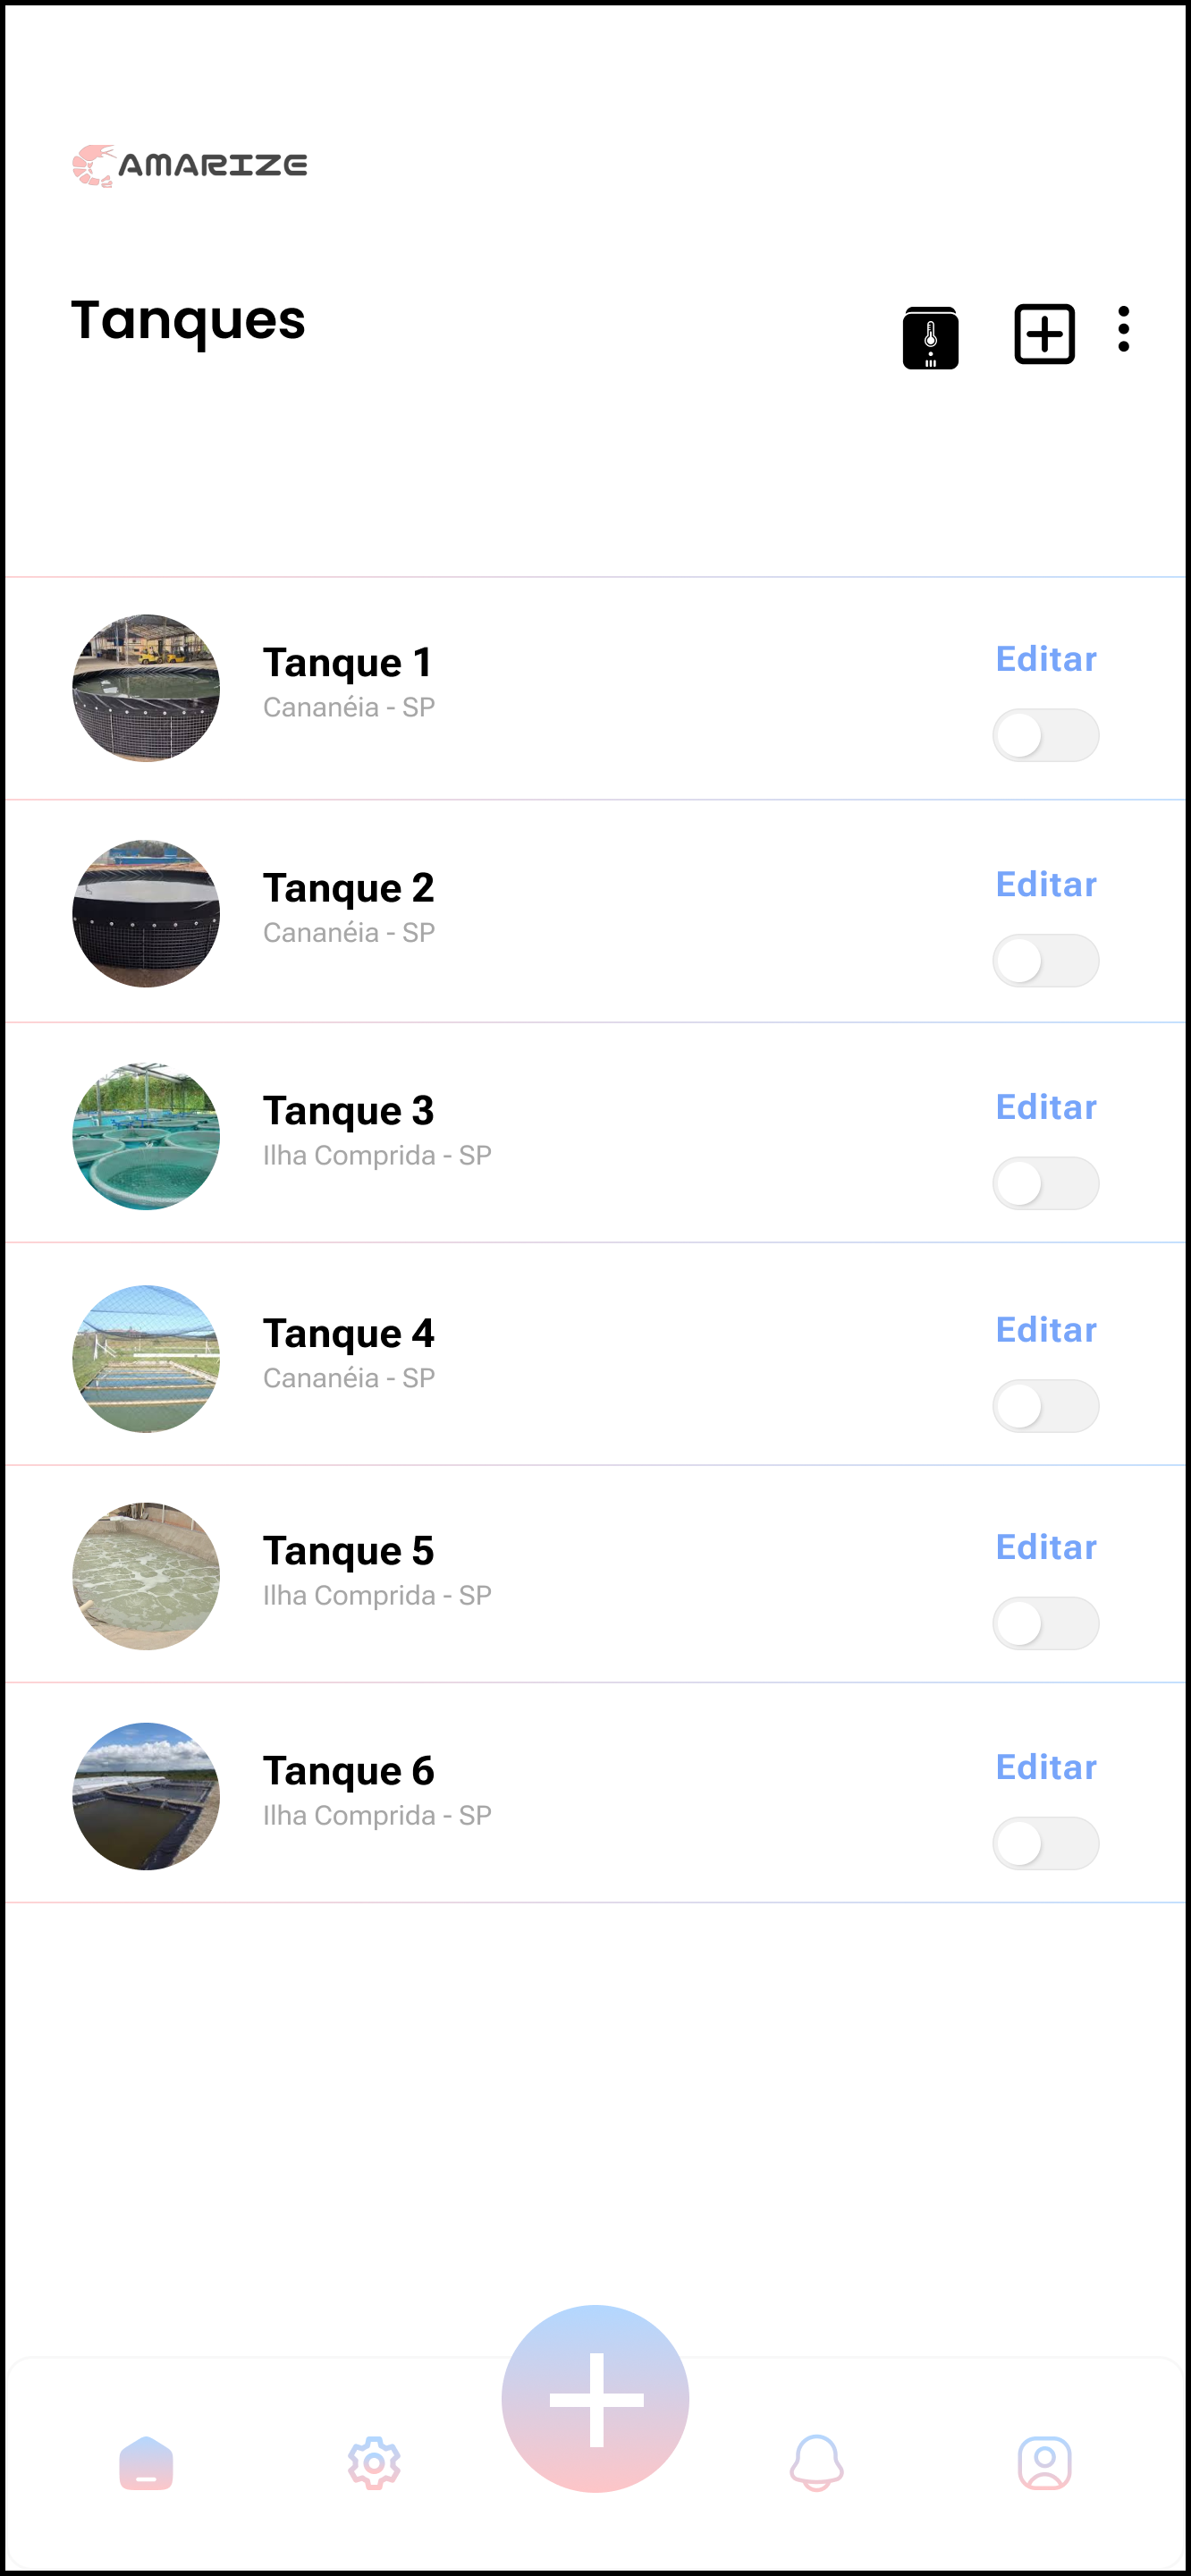
\includegraphics[width = 0.5\textwidth]{Imagem/Lista_Tanques.png}
\SourceOrNote{Autoria Própria, 2024}
\end{figure}

\newpage

Na Figura 3, é representada a tela de dashboard, esta tela pode ser visualizada após selecionar um tanque para verificar informações. Nesta tela, é possível verificar a temperatura do cativeiro, o pH, a amônia e dentre outras informações como camarões. É possível verificar um gráfico com registro de temperatura e pH de datas recentes.

\begin{figure}[!htb]
\centering
\SetCaptionWidth{\ifbool{@LayoutA}{0.7}{0.72}\linewidth}
\caption{Dashboard}%
\label{fig:tela-dashboard}
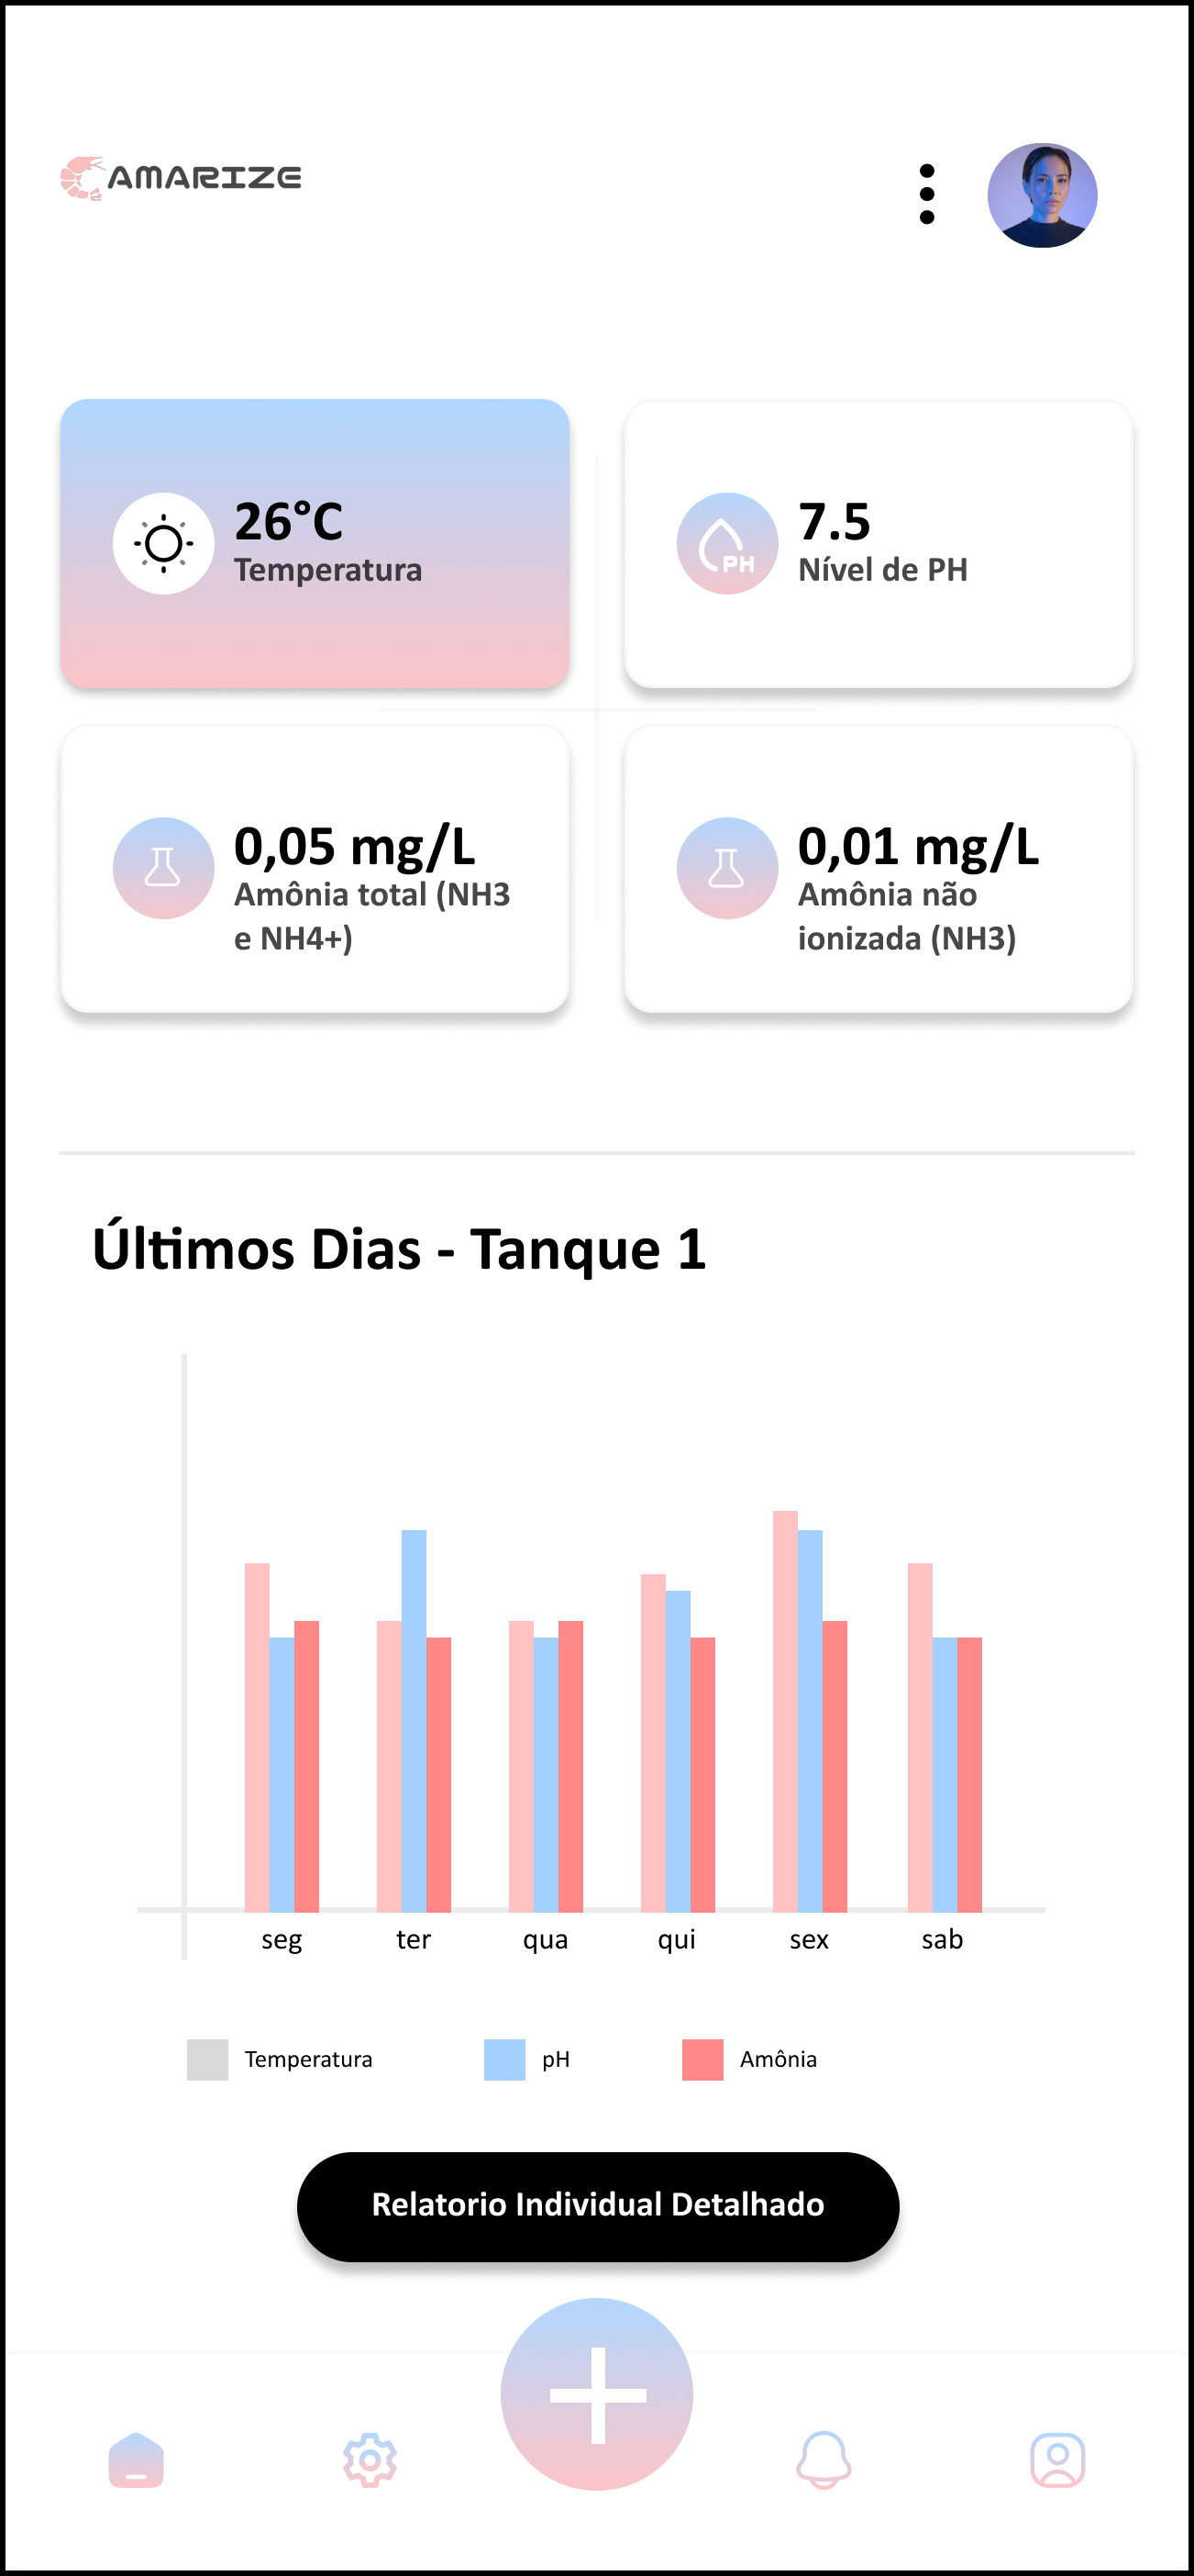
\includegraphics[width = 0.5\textwidth]{Imagem/Dashboard.png}
\SourceOrNote{Autoria Própria, 2024}
\end{figure}

\newpage

Na Figura 4, é representada a tela de equipamentos presentes em cada tanque, sendo possível editar as informações presentes e excluir.

\begin{figure}[!htb]
    \centering
    \SetCaptionWidth{\ifbool{@LayoutA}{0.7}{0.72}\linewidth}
    \caption{Equipamentos}%
    \label{fig:sistema}
    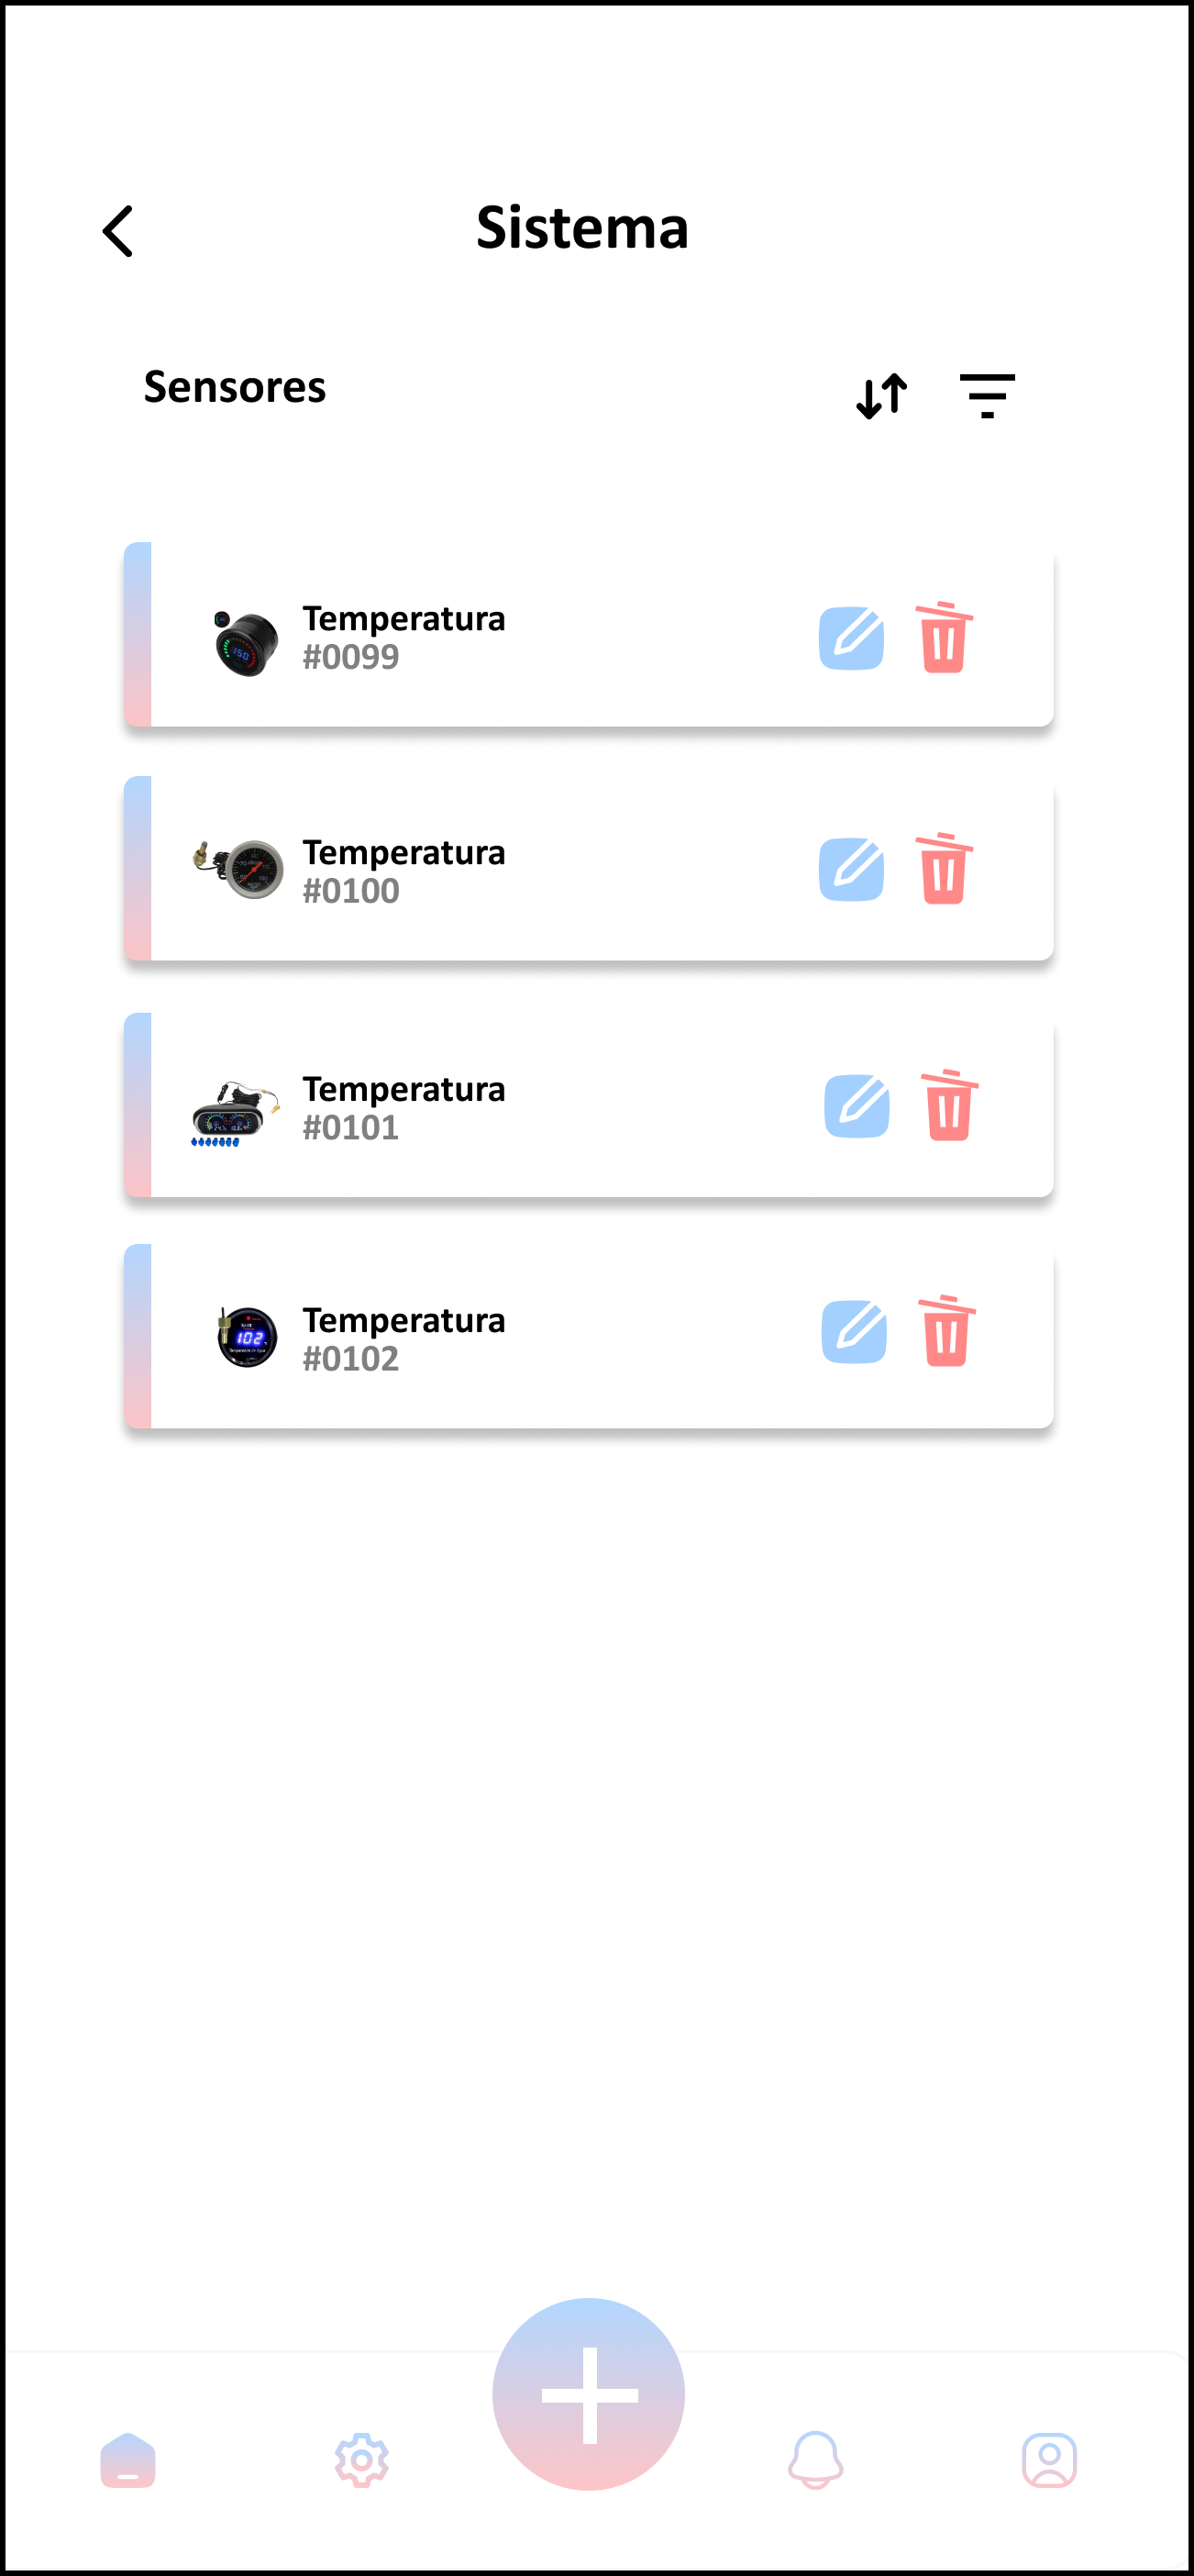
\includegraphics[width = 0.5\textwidth]{Imagem/Sistema.png}
    \SourceOrNote{Autoria Própria, 2024}
\end{figure}

\newpage

Na Figura 5, demonstra a tela de cadastro de sensor, onde é possível inserir o tipo de sensor, podendo ser sensor de temperatura, amônia e pH e uma foto para identificação do mesmo.

\begin{figure}[!htb]
    \centering
    \SetCaptionWidth{\ifbool{@LayoutA}{0.7}{0.72}\linewidth}
    \caption{Itens}%
    \label{fig:sensor}
    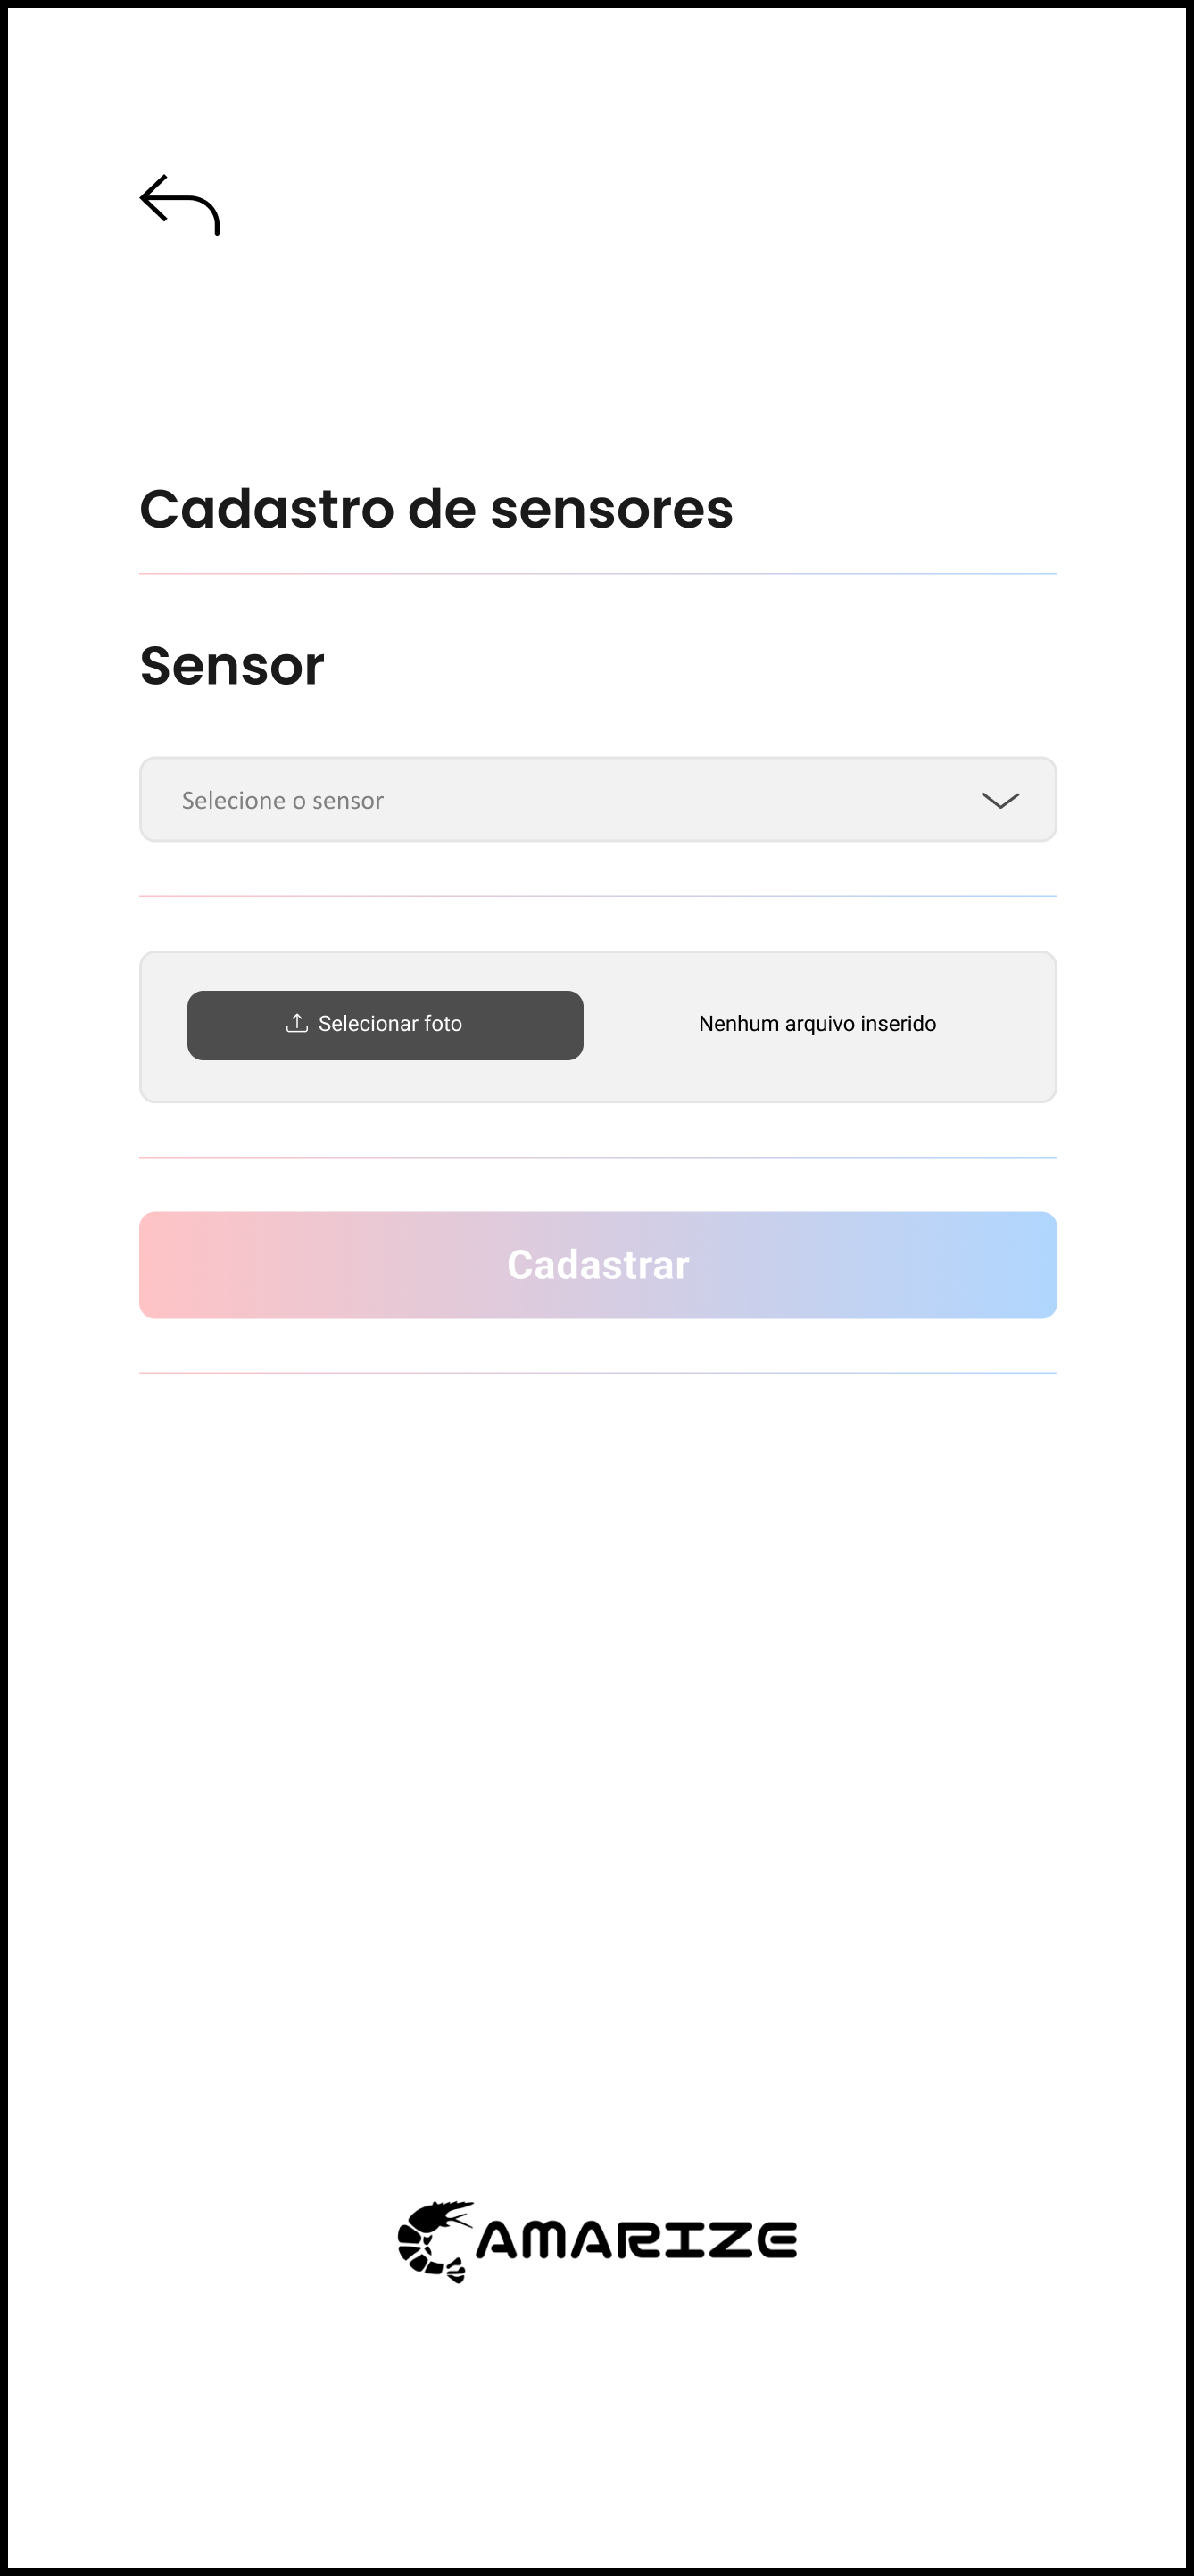
\includegraphics[width = 0.5\textwidth]{Imagem/Cadastrar_Sensor.png}
    \SourceOrNote{Autoria Própria, 2024}
\end{figure}

\newpage

Na Figura 6, é demonstrada a tela de cadastro de cada tanque, onde é selecionado o código de identificação do cativeiro, código de identificação do sítio e a data em que foi realizada a instalação do sistema.

\begin{figure}[!htb]
\centering
\SetCaptionWidth{\ifbool{@LayoutA}{0.7}{0.72}\linewidth}
\caption{Cadastro de Cativeiro}%
\label{fig:tela-cativeiro}
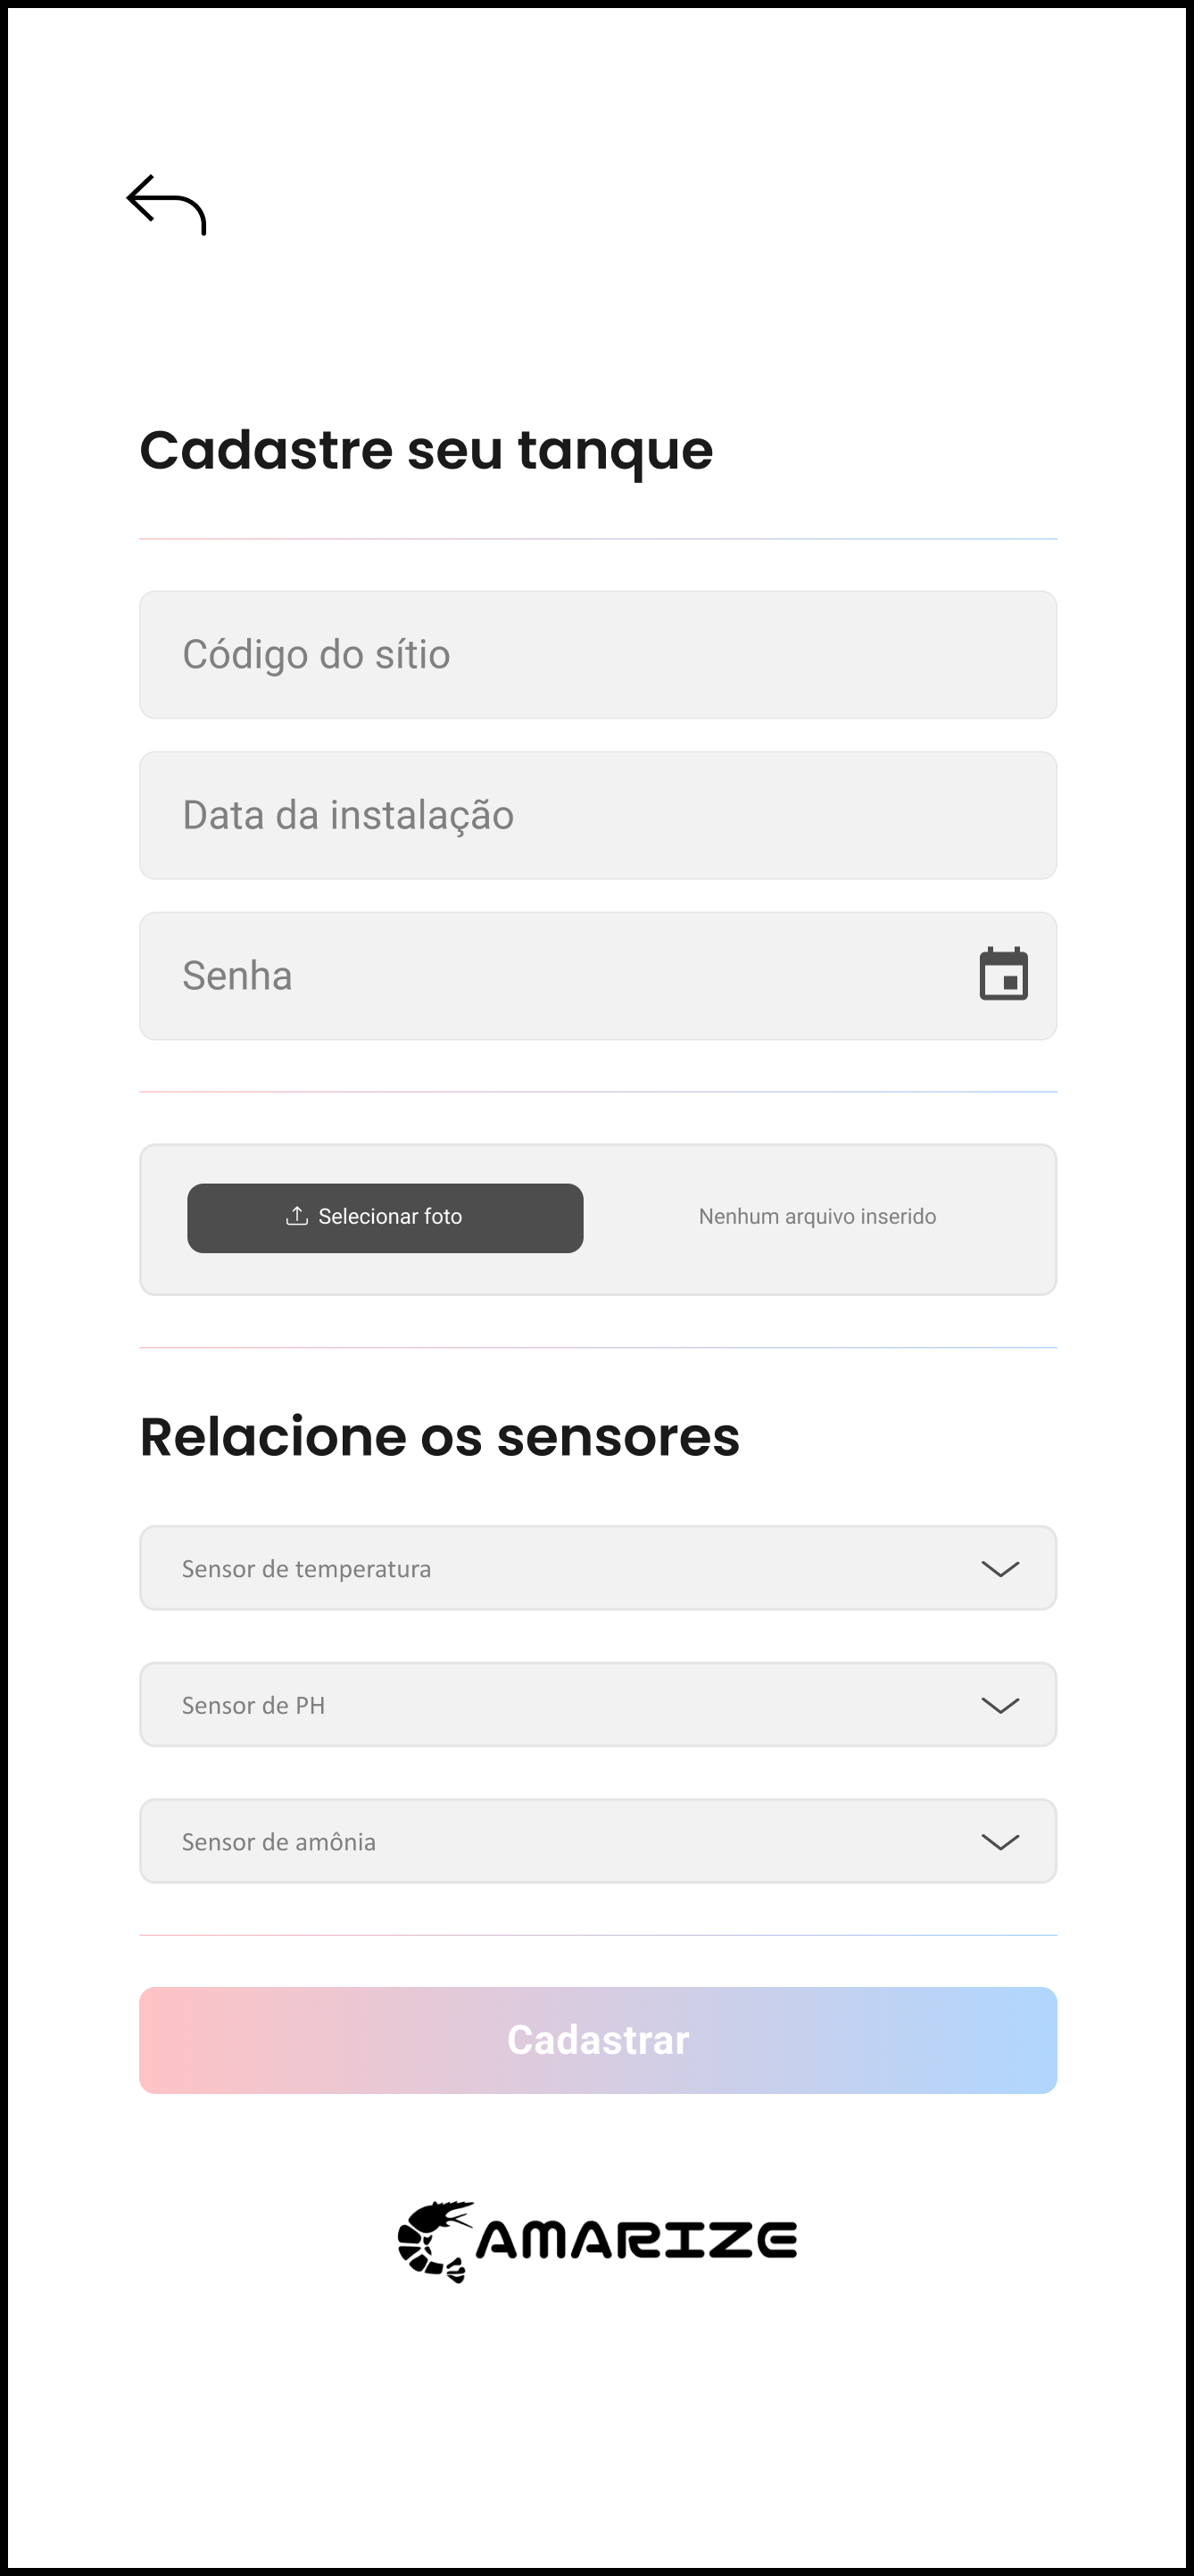
\includegraphics[width = 0.5\textwidth]{Imagem/Cadastrar_Cativeiro.png}
\SourceOrNote{Autoria Própria, 2024}
\end{figure}

\newpage

Na Figura 7, é apresentada a tela de notificações. O sistema irá notificar o usuário para caso ocorra algum tipo de mudança repentina em um dos cativeiros.

\begin{figure}[!htb]
    \centering
    \SetCaptionWidth{\ifbool{@LayoutA}{0.7}{0.72}\linewidth}
    \caption{Notificações}%
    \label{fig:notificações}
    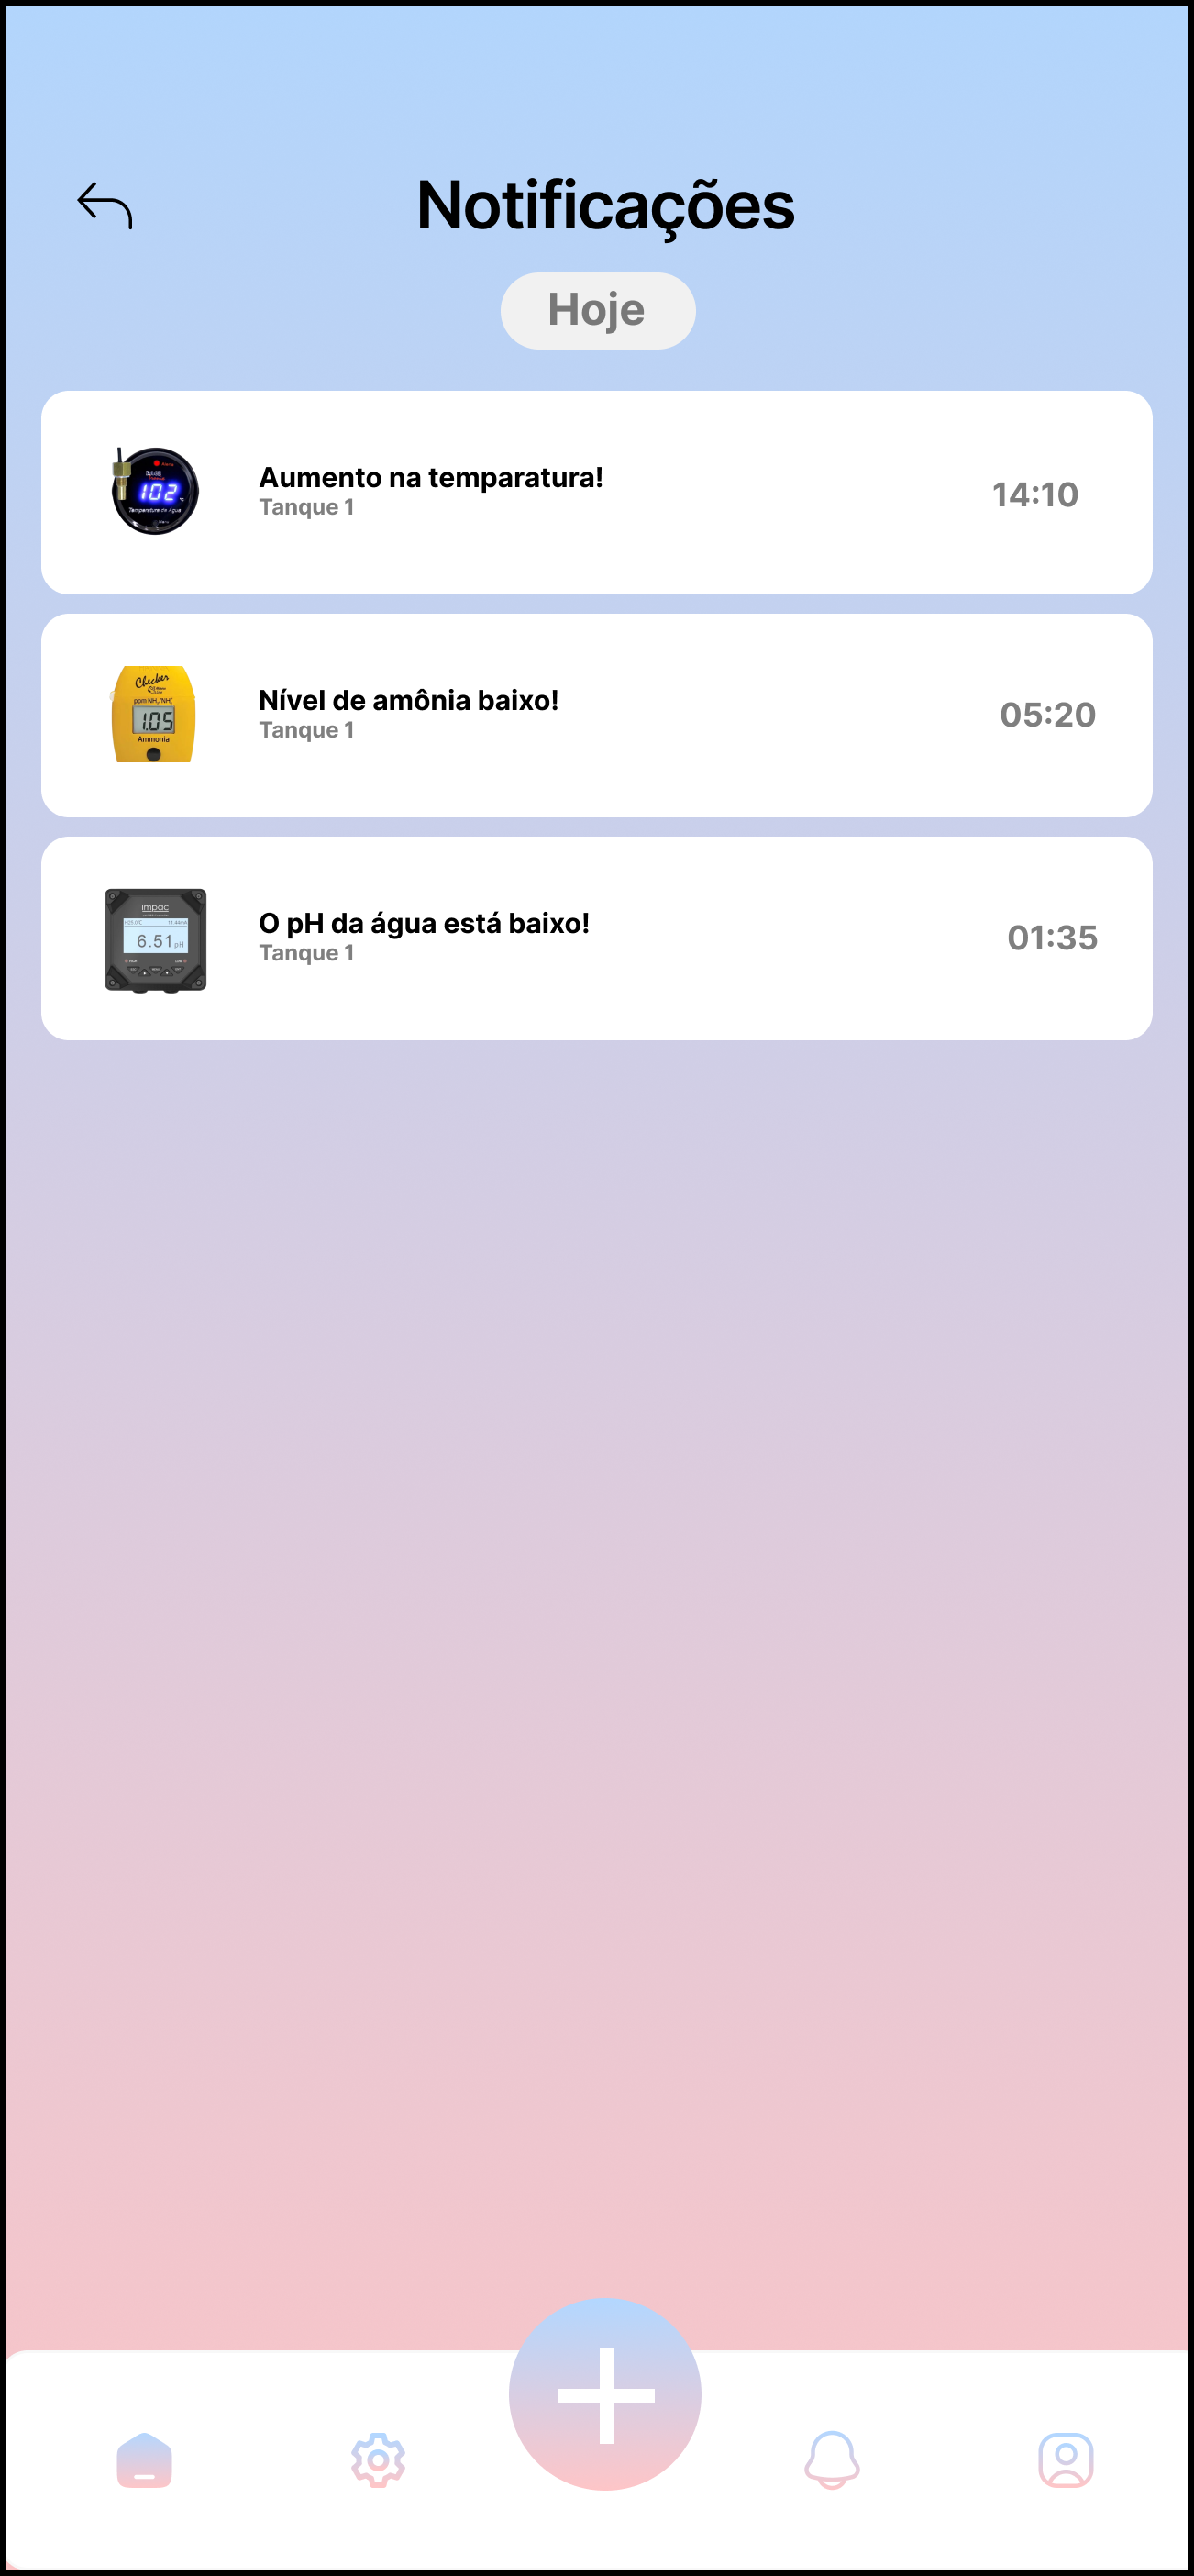
\includegraphics[width = 0.5\textwidth]{Imagem/Notificações.png}
    \SourceOrNote{Autoria Própria, 2024}
\end{figure}
    
\newpage

Na Figura 8, é demonstrada a tela de opções de relatório, onde é possível retirar relatórios sobre cada um dos tanques individualmente e de todos os tanques, sendo selecionado o período como semanal, mensal e anual.

\begin{figure}[!htb]
    \centering
    \SetCaptionWidth{\ifbool{@LayoutA}{0.7}{0.72}\linewidth}
    \caption{Relatórios}%
    \label{fig:relatório}
    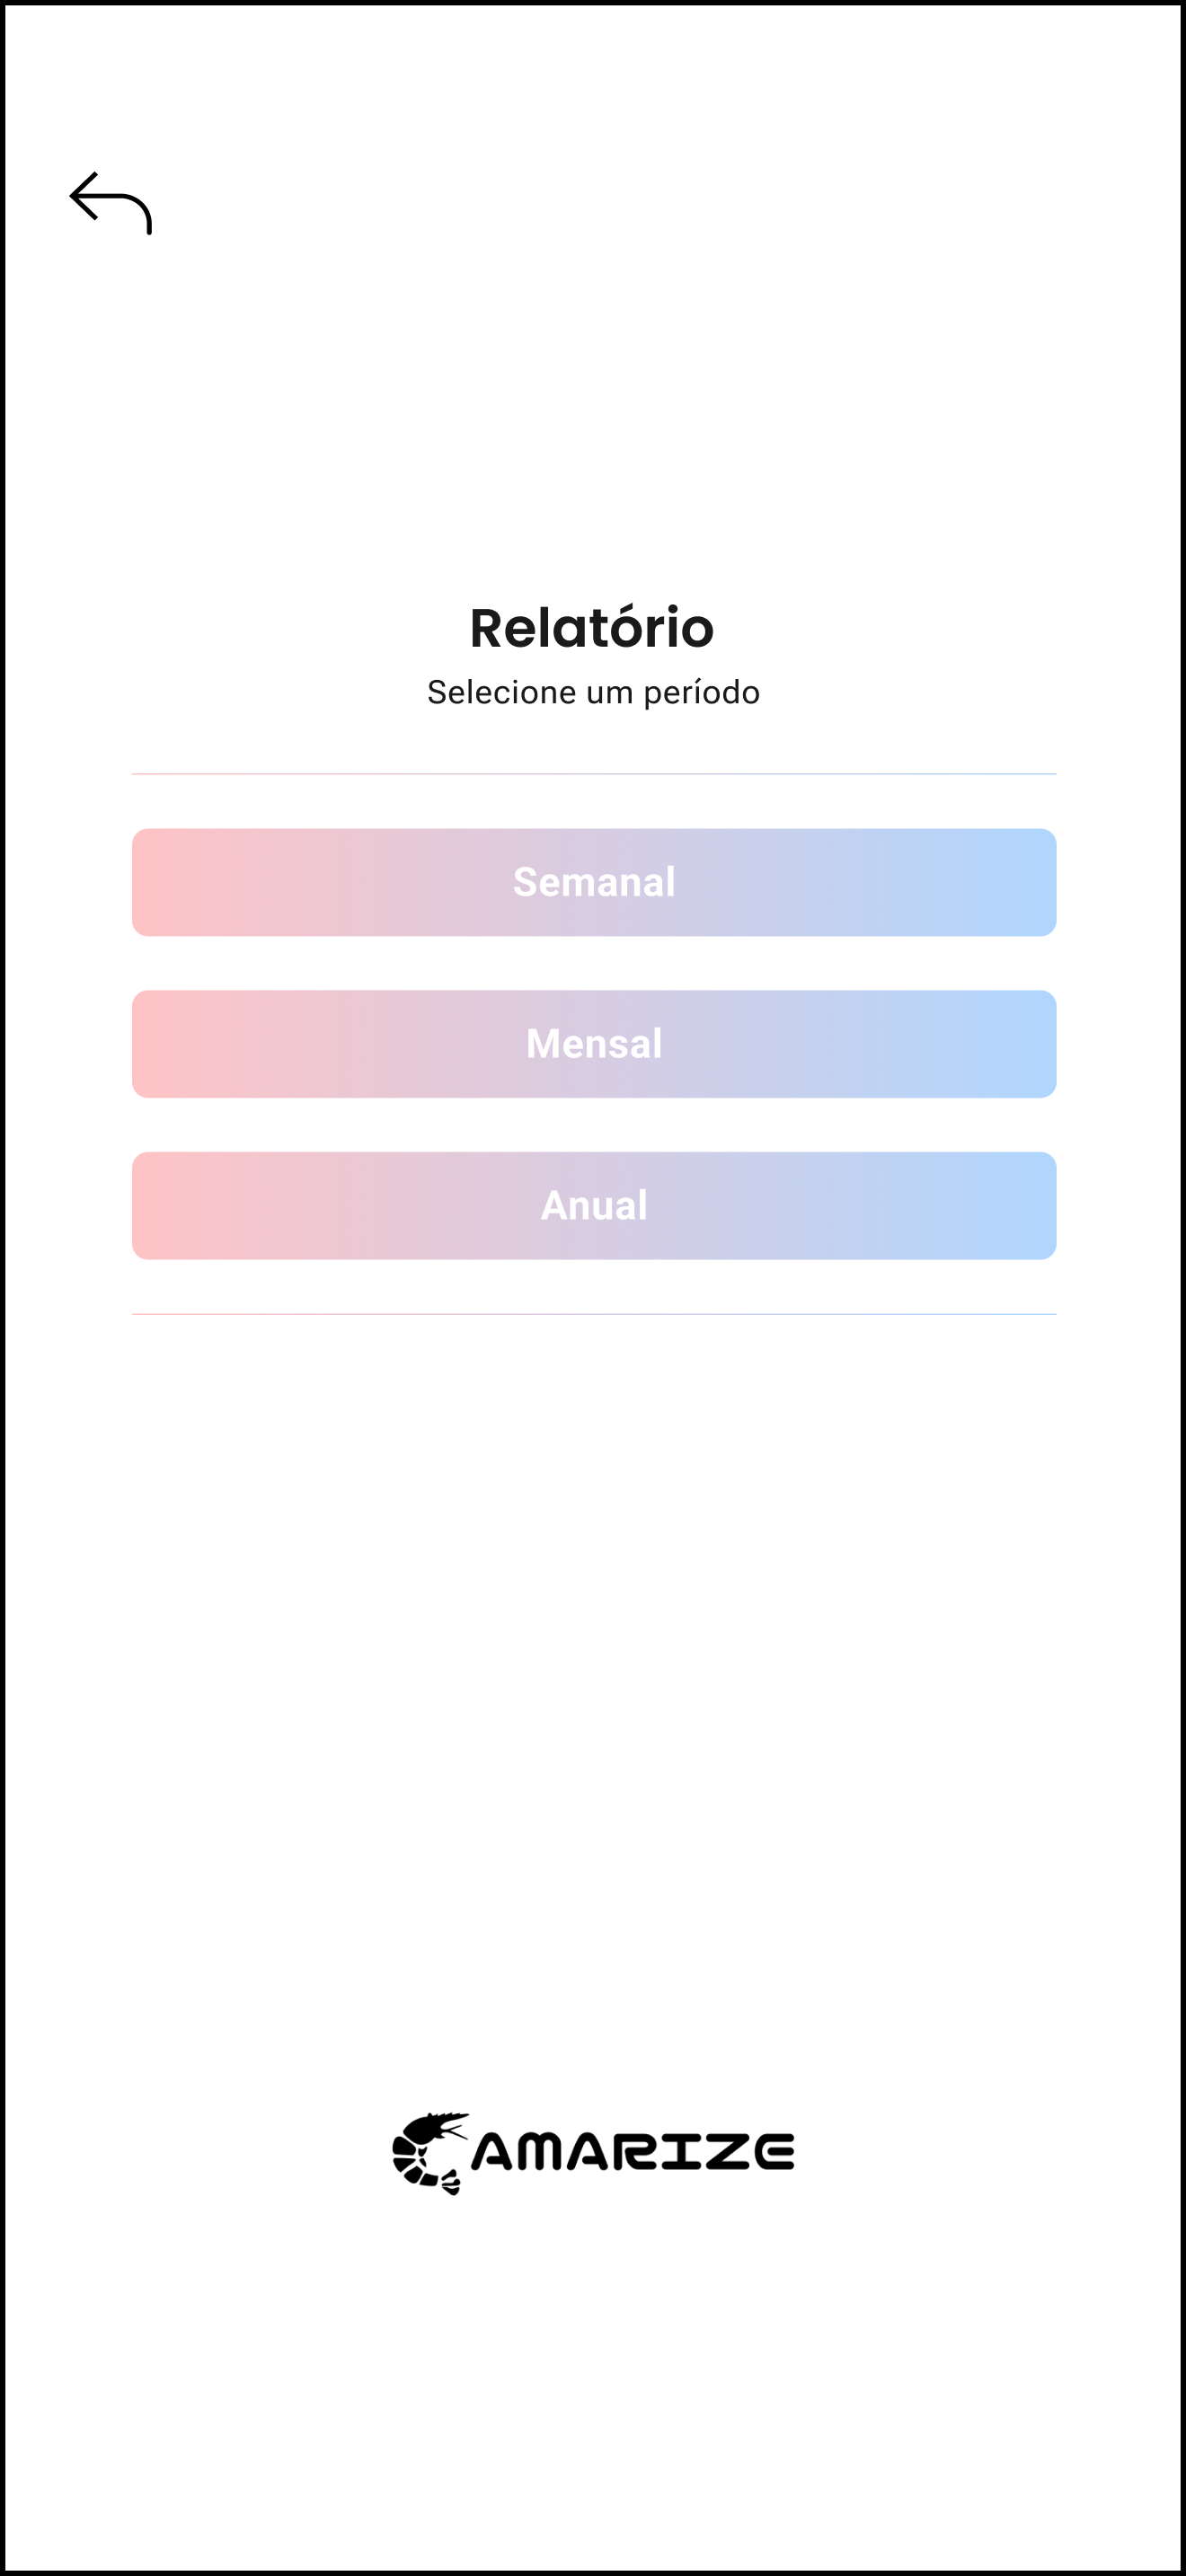
\includegraphics[width = 0.5\textwidth]{Imagem/Opções_Relatório.png}
    \SourceOrNote{Autoria Própria, 2024}
\end{figure}
    
\newpage

Na figura 9, apresenta um modelo de relatório, mostrando uma foto do cativeiro, o período selecionado e um resumo apresentando os dados e informações referentes ao tanque.

\begin{figure}[!htb]
    \centering
    \SetCaptionWidth{\ifbool{@LayoutA}{0.7}{0.72}\linewidth}
    \caption{Relatórios}%
    \label{fig:exemplo_relatório}
    \includegraphics[width = 0.5\textwidth]{Imagem/Relatório.png}
    \SourceOrNote{Autoria Própria, 2024}
\end{figure}
    
\newpage

\subparagraph*{\textbf{Desenvolvimento da aplicação}}

Por base nas telas mencionadas, foi realizado o desenvolvimento de nossa aplicação web. A aplicação foi desenvolvida por meio da linguagem JavaScript e a plataforma Node.js. A criação de um servidor HTTP se deu por meio da integração com o framework Express. Para realizar a renderização das telas HTML, foi feito uso do EJS (Embedded JavaScript).

Para armazenar as senhas de nossos usuários de maneira segura, foi utilizado a biblioteca ByCrypt. Essa bilbioteca fornece de um modo fácil e seguro o armazenamento de senhas utilizando um algoritmo denominado de Hash Forte e uma técnica chamada "Salting". Para cuidar da parte do banco de dados, se utilizou o Sequelize. O Sequelize permite a criação de modelos em JavaScript que representam o banco de dados, podendo assim manipular os dados utilizando objetos e métodos.

Para gerenciar as sessões dos usuários e integração de métodos de autenticação, foi utilizado o middleware Express-Session, que armazena os dados da sessão no servidor.

Com o objetivo de manter a organização do código, foi feito uso do modelo de arquitetura MVC (Model, View, Control). Model é resposnável por lidar com os dados e regras impostas na aplicação, View é responsável por lidar com a interação com usuários e os dados que são fornecidos, Control atua como um intermediário entre Model e View, processando as solicitações e manipulação de dados.

Para facilitar a navegação do usuário, foram implementadas rotas. As rotas cuidam dos pontos de acesso da aplicação, mapeando as requisições HTTP para determinadas funções, permitindo com que o usuário interaja com cada parte desenvolvida na aplicação.

\subparagraph*{\textbf{Diagrama de Caso de Uso}}

Com o Diagrama de Caso de Uso (DCU) apresentada na figura 10, é possível verificar as interações entre o usuário, visto como o carcinicultor, e o sistema. Essas interações incluem desde a realização da conta até a analise completa de cada funcionalidade do sistema, como relatório geral, visualização dos tanques e utilização do modo automático de alimentação.

\begin{figure}[!htb]
\centering
\SetCaptionWidth{\ifbool{@LayoutA}{0.7}{0.72}\linewidth}%
\caption{Diagrama de Caso de Uso}%
\label{fig:caso-uso}
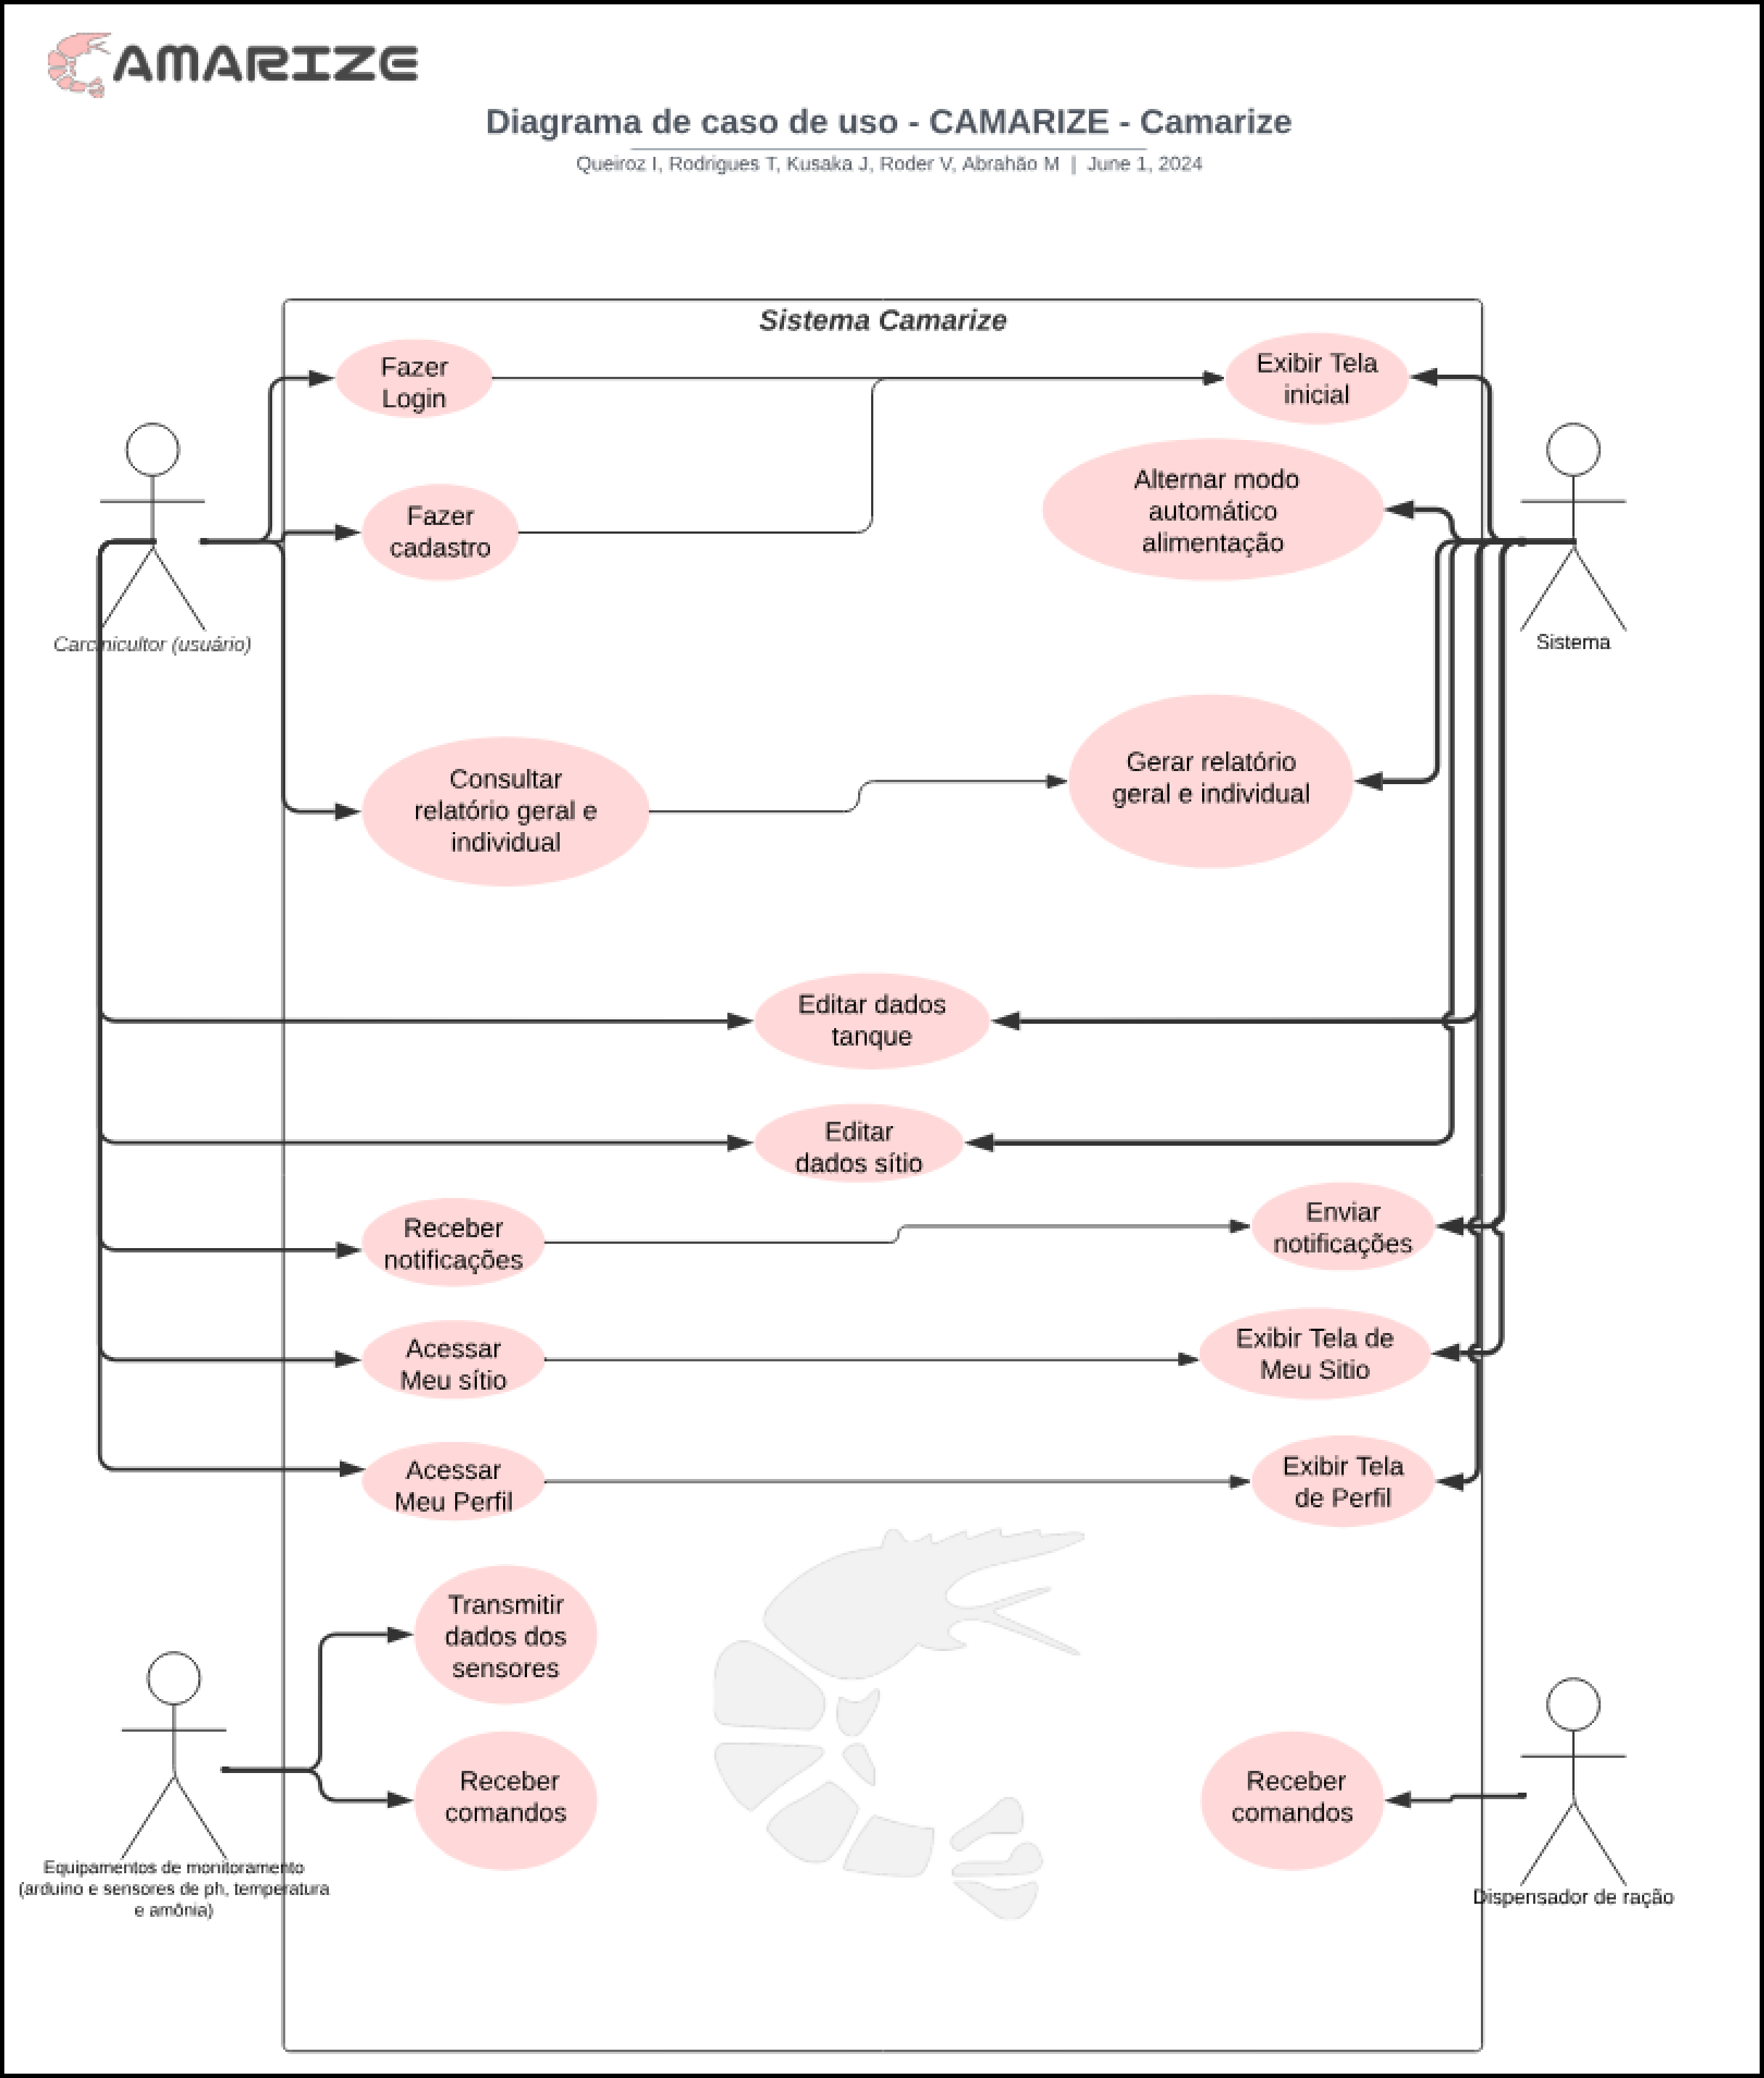
\includegraphics[width = 1.3\CaptionWidth]{Imagem/Caso de Uso.png}
\SourceOrNote{Autoria Própria, 2024}
\end{figure}

\newpage

\subparagraph*{\textbf{Diagrama de Classe}}

Com o Diagrama de classe na figura 11, pode-se ter noção das funcionalidades e atributos que estão presentes dentro do sistema, partindo de funcionalidades simples até mais complexas, podendo entender suas ligações entre cada uma das classes.    

    \begin{figure}[!htb]
        \centering
        \SetCaptionWidth{\ifbool{@LayoutA}{0.7}{0.72}\linewidth}%
        \caption{Diagrama de Classe}%
        \label{fig:classe}
        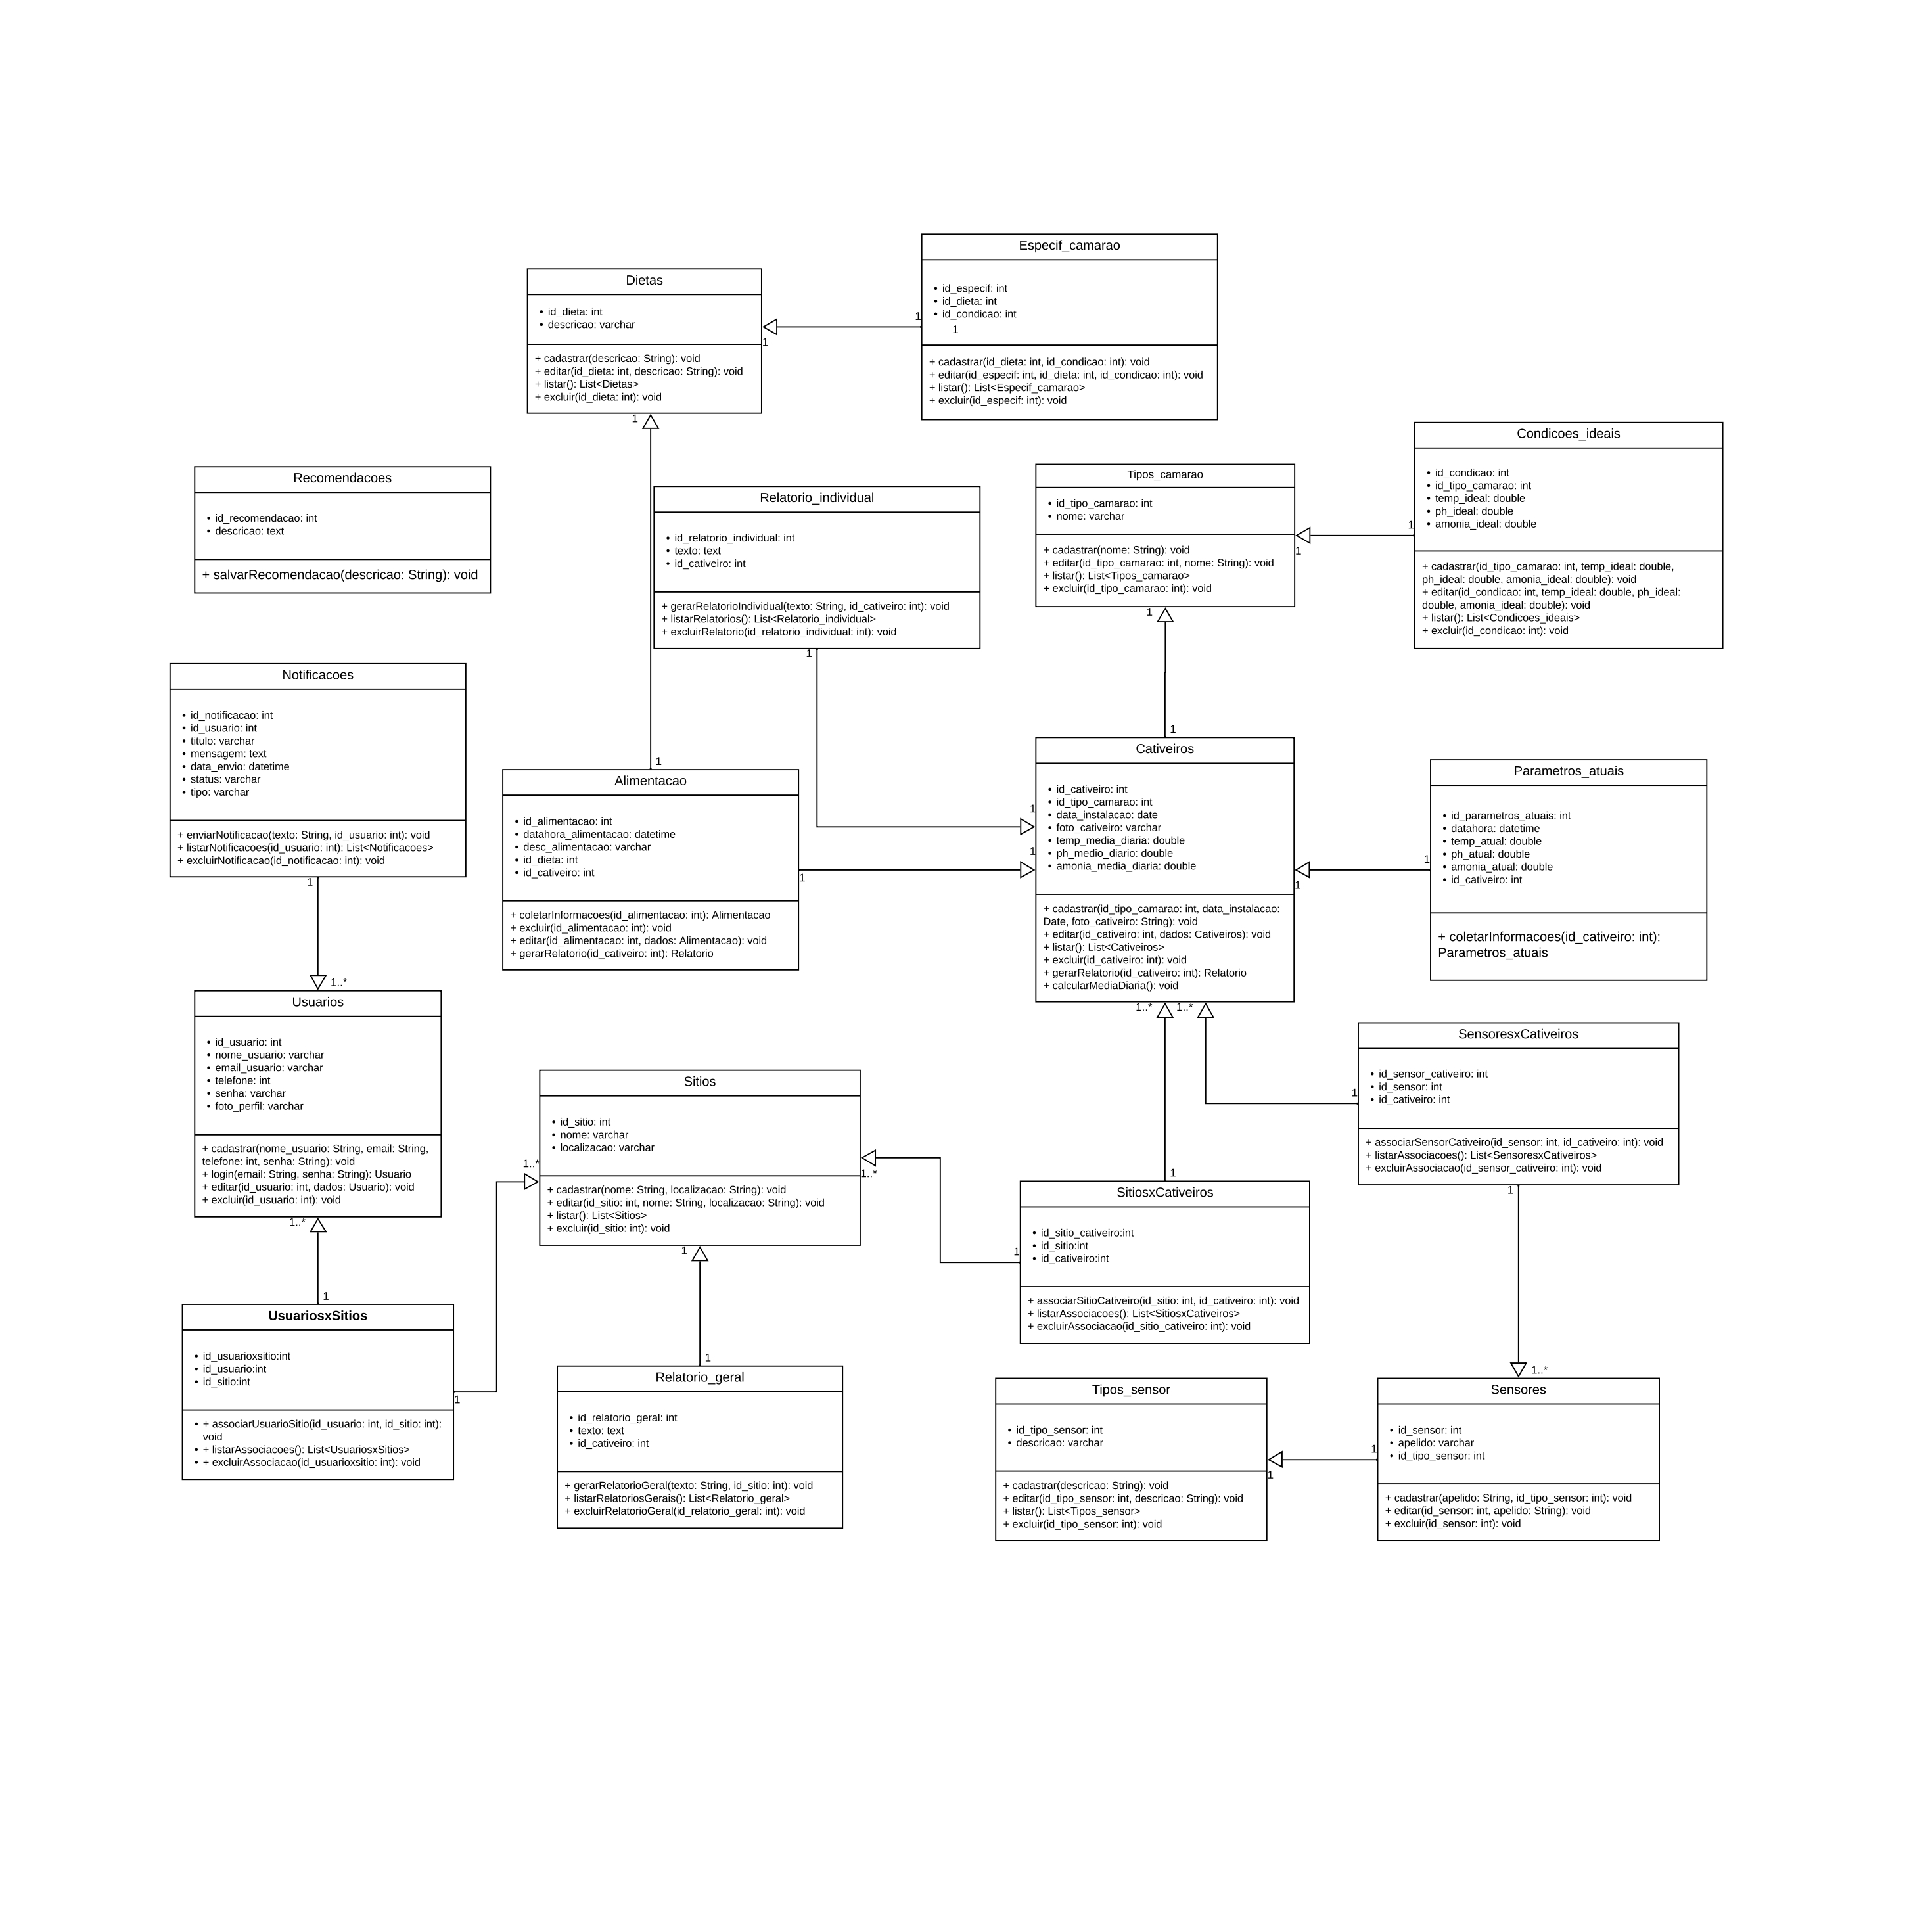
\includegraphics[width = 1.6\CaptionWidth]{Imagem/Diagramas de Classe.jpg}
        \SourceOrNote{Autoria Própria, 2024}
    \end{figure}

\newpage

\subparagraph*{\textbf{Diagrama de Objetos}}

Com base no Diagrama de objetos na figura 12, é possível visualizar situações específicas do sistema, apresentando situações específicas do sistema, mostrando como os objetos se interagem e colaboram em uma situação real.

\begin{figure}[!htb]
    \centering
    \SetCaptionWidth{\ifbool{@LayoutA}{0.7}{0.72}\linewidth}%
    \caption{Diagrama de Objetos}%
    \label{fig:objetos}
    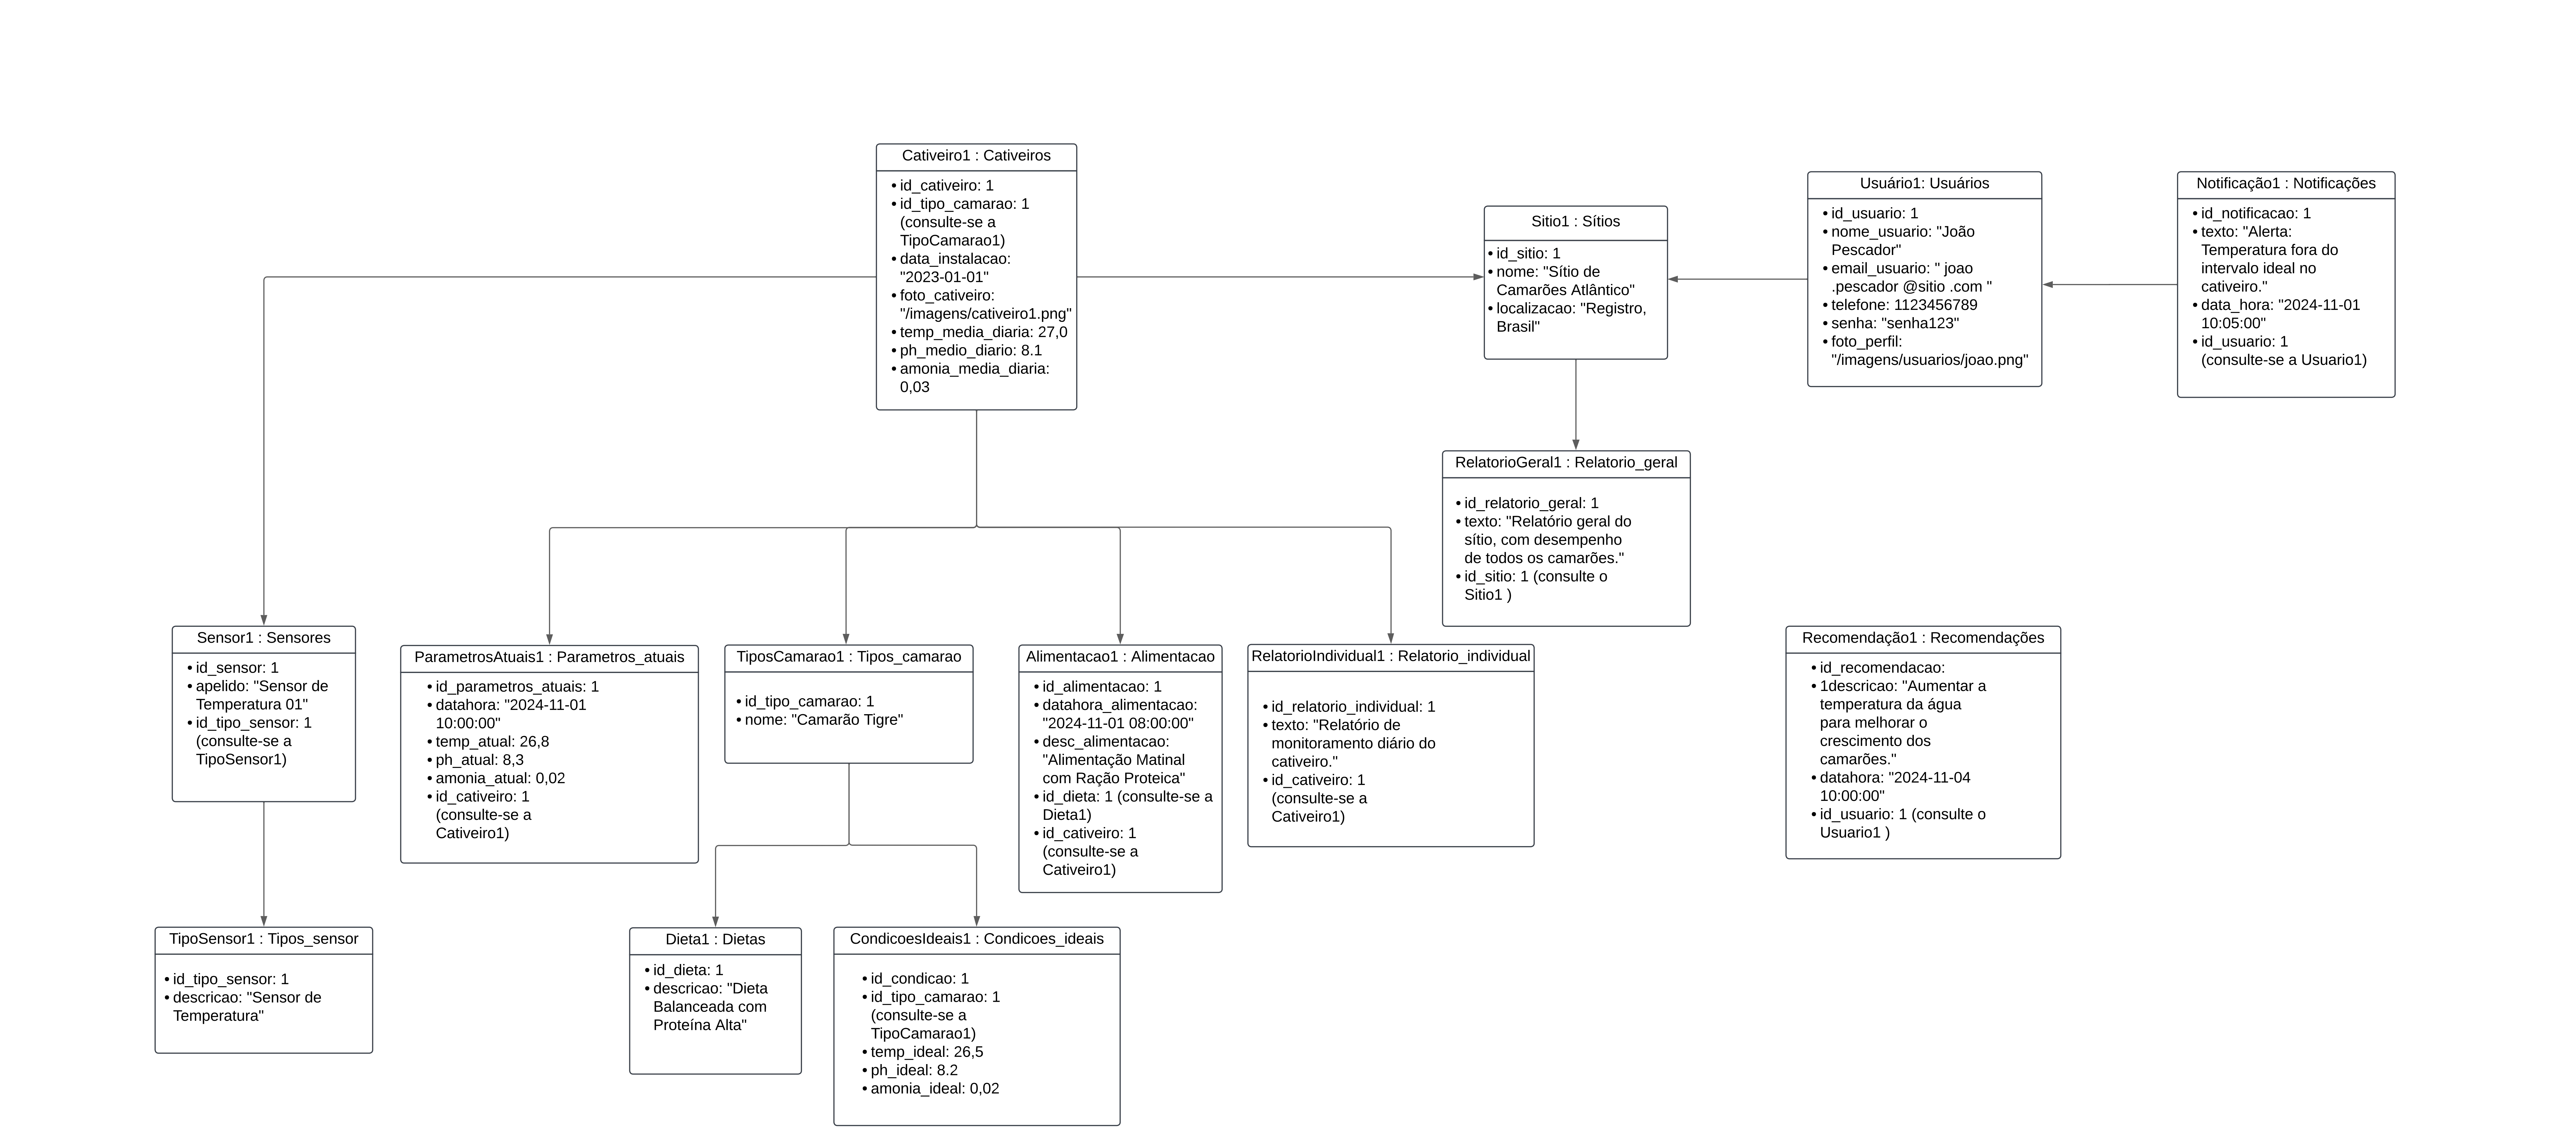
\includegraphics[width = 1.6\CaptionWidth]{Imagem/Diagrama de Objetos.jpg}
    \SourceOrNote{Autoria Própria, 2024}
\end{figure}

\newpage


\subparagraph*{\textbf{Modelagem Lógica, Conceitual e Física do Banco de Dados}}

O banco de dados tem um papel de extrema importância para as informações, sendo necessário para guardar, organizar e recuperar dados. O Modelo Lógico e Conceitual são maneira de demonstrar a eficiência de um banco de dados.

A modelagem conceitual, lógica e física, representadas na Figura 13, Figura 14 e Figura 15, demonstram a funcionalidade do programa e do que será aplicado no banco de dados. A visão gráfica do banco de dados se demonstra algo fundamental, por conta que proporciona o máximo de detalhes com extrema clareza, apresentando as relações entre as entidades.

No modelo conceitual, Camarões está ligado com Cativeiro por meio de Tipos de Camarões, apresentando característica como espécie e peso. Com os Cativeiros fazendo parte de Sítios, pode-se realizar o Monitoramento por meio de Sensores e controlar a Alimentação dos camarões. O Monitoramento possui Temperatura, pH e Amônia fazendo assim o registro de cada um. Alimentação possui o horário que foi realizado a alimentação e a quantidade de alimento fornecida para cada Cativeiro.

No modelo lógico, é apresentado uma representação mais concreta do banco de dados, demonstrando as tabelas, entidades, chaves primárias e estrangeiras e seus relacionamentos.

No modelo físico, demonstra uma versão refinada do modelo conceitual, representando restrições de dados, nomes de entidades e relacionamentos para implementação de forma independente.

    \newpage

    \begin{figure}[!htb]
    \SetCaptionWidth{\ifbool{@LayoutA}{0.7}{0.72}\linewidth}
    \caption{Modelo Conceitual}%
    \label{fig:conceitual}
    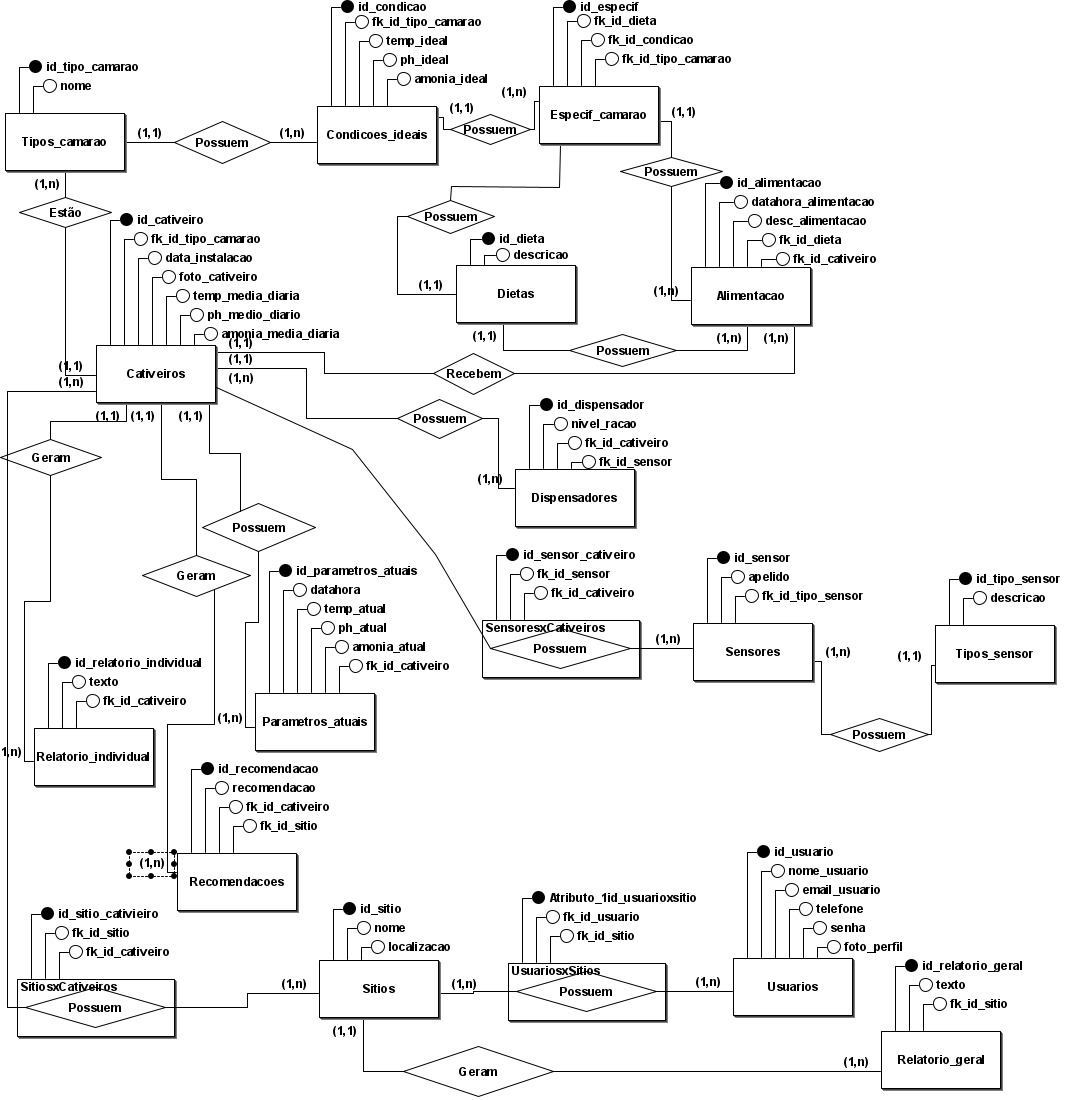
\includegraphics[width = 1\CaptionWidth]{Imagem/Modelo Conceitual.jpeg}
    \SourceOrNote{Autoria Própria, 2024}
    \end{figure}

    \newpage

    \begin{figure}[!htb]
    \SetCaptionWidth{\ifbool{@LayoutA}{0.7}{0.72}\linewidth}
    \caption{Modelo Lógico}%
    \label{fig:logico}
    \includegraphics[width = 1.3\CaptionWidth]{Imagem/Modelo Lógico.png}
    \SourceOrNote{Autoria Própria, 2024}
    \end{figure}

    \newpage

    \begin{figure}[!htb]
    \SetCaptionWidth{\ifbool{@LayoutA}{0.7}{0.72}\linewidth}
    \caption{Modelo Físico}%
    \label{fig:fisico}
    \includegraphics[width = 1.3\CaptionWidth]{Imagem/Modelo Físico.jpg}
    \SourceOrNote{Autoria Própria, 2024}
    \end{figure}

\subparagraph*{\textbf{Modelo de Negócio Canvas}}

O modelo de negócios Canvas foi utilizado para análise econômica do sistema. Por meio do Canvas foi possível identificar os Parceiros, Recursos e Atividades Chaves, nossas Propostas de Valor, Segmento de Mercado, nossa Fonte de Renda e Estrutura de Custos.

\newpage

    \begin{figure}[!htb]
        \centering
        \SetCaptionWidth{\ifbool{@LayoutA}{0.7}{0.72}\linewidth}
        \caption{Canvas}%
        \label{fig:canvas}
        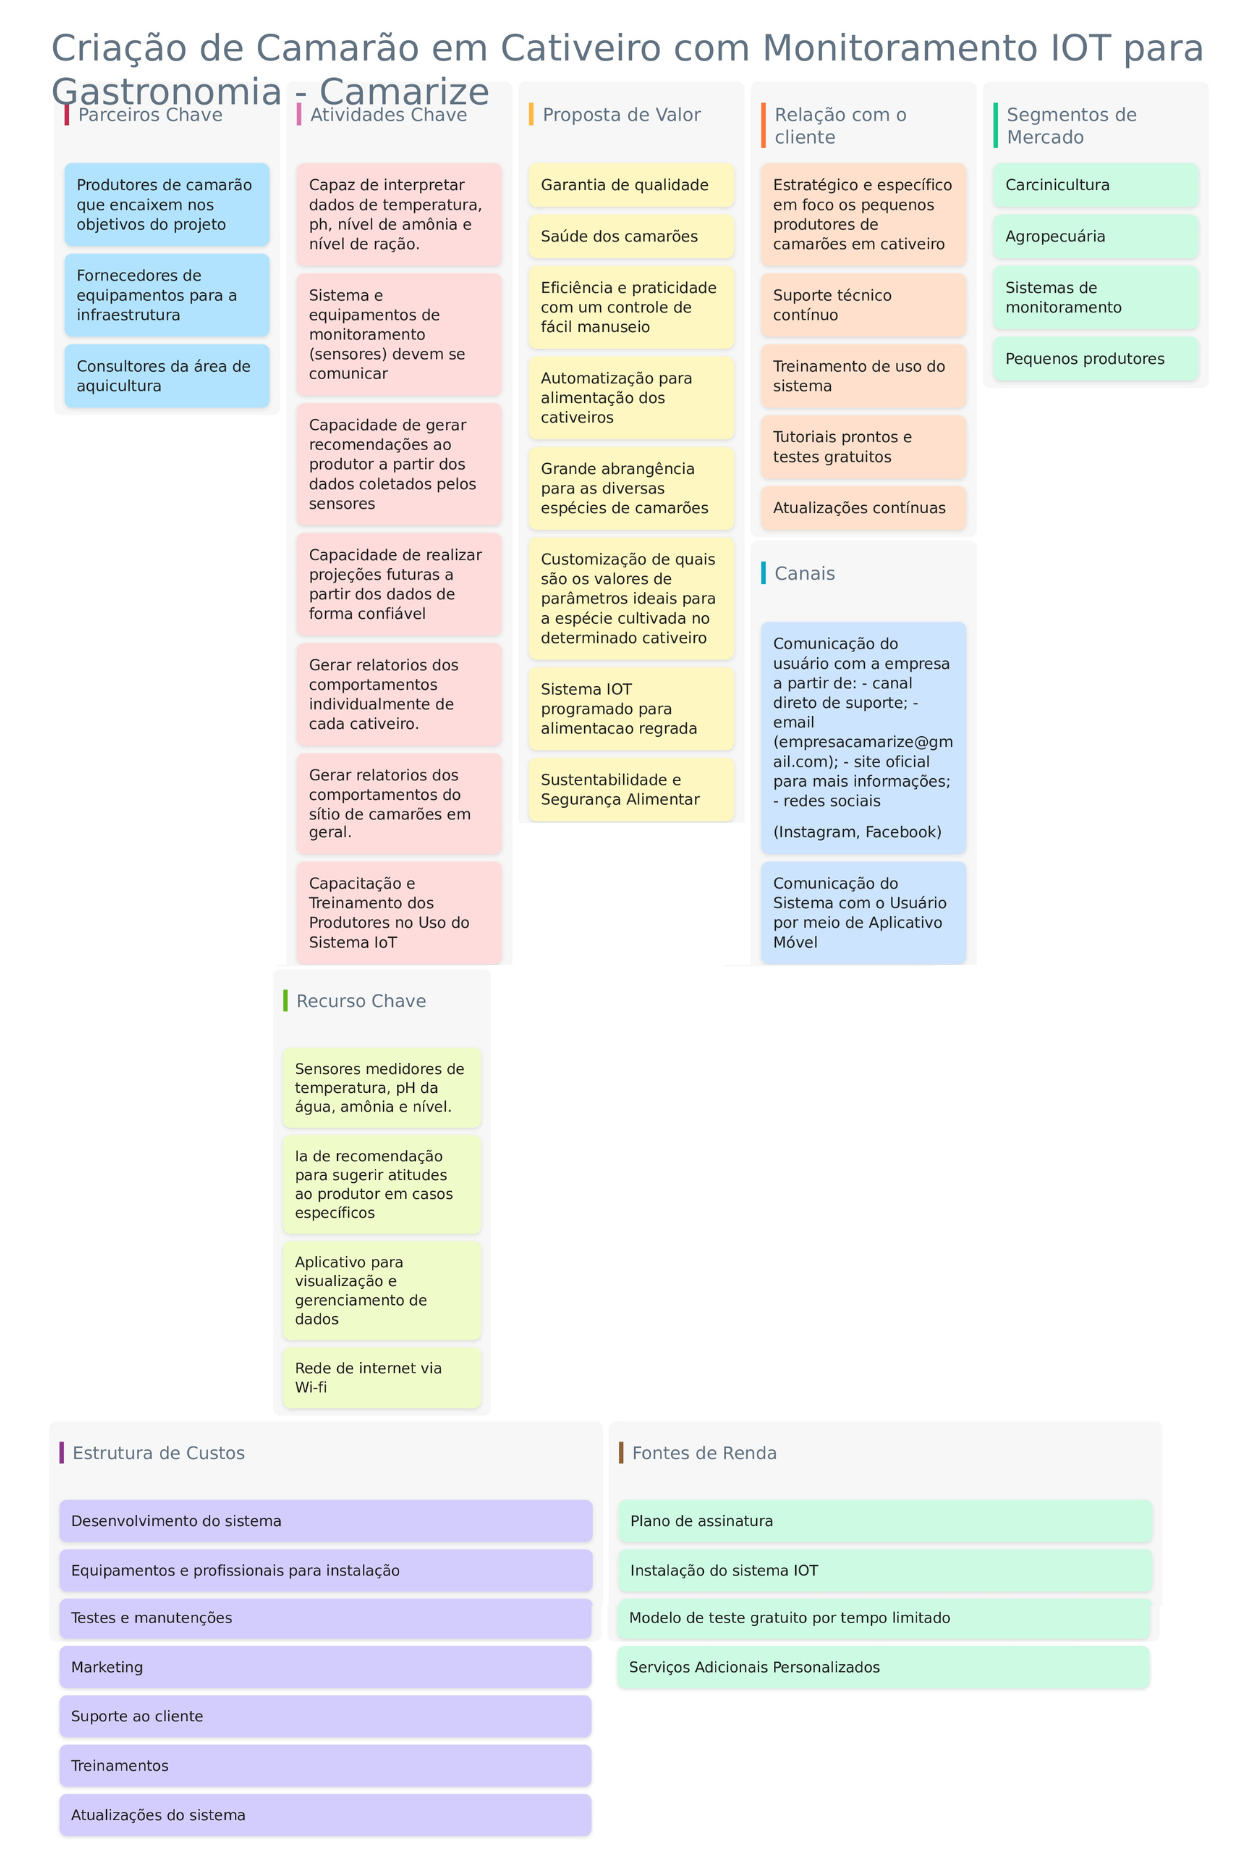
\includegraphics[width = 1.1\CaptionWidth]{Imagem/Canvas.png}
        \SourceOrNote{Autoria Própria, 2024}
    \end{figure}

\newpage

\subparagraph*{\textbf{Análise de recorrência do algoritmo Merge Sort}}

O Merge Sort é um algoritmo de ordenação que consiste em dividir uma estrutura de subconjuntos e aplicar a ordenação nos elementos que são extraídos da estrutura primária. Após a ordenação dos subconjuntos, é realizada a mistura para um conjunto final ordenado.

O melhor tempo ocorre quando todos os elementos do array já estão ordenados, o Merge Sort sempre executa a divisão e a fusão, independente  da ordem dos elementos. O tempo de execução, representado por \( O(n \log_2 n) \), pode ser explicado da seguinte forma: \( \log_2 n \) corresponde ao número de divisões do array até que cada subarray contenha apenas um elemento, e \( n \) refere-se ao número de comparações e fusões realizadas durante o processo de merge.

O tempo médio ocorre quando os elementos estão em ordens aleatórias, em seu comportamento o número de divisões e fusões não dependem da ordem dos elementos, cada nível realiza \( n \) operações no total e possui \( \log_2 n \) níveis. Sua representação é semelhante com o melhor tempo: \( O(n \log_2 n) \).

O pior tempo ocorre quando o array está em ordem oposta a esperada, sua complexidade não é alterada por conta que sua quantidade de execuções não são alteradas. Sua representação se mantém a mesma, sendo ela: \( \log_2 n \).

Na aplicação, foi utilizada na tela de sensores, sendo utilizado para organizar os sensores de forma crescente e decrescente. Seu tempo de execução foram exatos 0.000000 milisegundos, mostrando a eficiência e rapidez do algoritmo. Sua representação matemática se apresenta desta maneira:

\[
\text{MergeSort}(n) =
\begin{cases}
0, & \text{se } n = 0 \\
0, & \text{se } n = 1 \\
2 \cdot \text{MergeSort}\left(\frac{n}{2}\right) + O(n), & \text{se } n > 1
\end{cases}
\]


\textbf {A representação em pseudocódigo:} 


\begin{verbatim}
    funcao mergeSort(arr[])

    // Função recursiva para ordenar o vetor usando o algoritmo MergeSort

    se tamanho de arr <= 1 então
        retornar arr
    fimse

    meio <- arredondar_para_baixo(arr.length / 2)
    esquerda <- mergeSort(arr[0, meio])
    direita <- mergeSort(arr[meio, arr.length])

    retornar merge(esquerda, direita)
fimfuncao

funcao merge(esquerda[], direita[])

    // Função para combinar dois vetores ordenados

    resultado <- lista_vazia
    indice_esquerda <- 0
    indice_direita <- 0

    enquanto indice_esquerda < tamanho de esquerda e 
    indice_direita < tamanho de direita faça
    se 
    esquerda[indice_esquerda].id_tipo_sensor > direita[indice_direita].id_tipo_sensor 
        então
            adicionar esquerda[indice_esquerda] em resultado
            indice_esquerda incrementa 1
        senão
            adicionar direita[indice_direita] em resultado
            indice_direita incrementa 1
        fimse
    fimenquanto

    retornar resultado concatenado com esquerda[indice_esquerda, arr.length] 
    e direita[indice_direita, arr.length]
fimfuncao
    \end{verbatim}


\section*{CONCLUSÃO}\label{sect:conclusao}

Este atual projeto tem a meta de cumprir as ODS 12 e ODS 14, que trabalham para a segurança da alimentação humana e proteção de animais marinhos e com os resultados obtidos contribuem para a realização destas metas. Com o monitoramento da água e dos camarões, é realizada a contribuição para boa qualidade e cuidado com o animal e com o meio ambiente, assim ajudando na carcinicultura e seu desenvolvimento.

Com os benefícios deste sistema, o usuário poderá desfrutar de uma plataforma confiável com bom gerenciamento de cada cativeiro de uma maneira simples e de fácil uso, dessa forma ajudando o produtor a controlar a temperatura, pH e amônia da água para o camarão estar em boas condições, além de ajudar na boa alimentação e fornecer dados a respeito de cada tanque e camarões para futuras comparações e análises.

Atualmente, o projeto está em fase de desenvolvimento e busca por melhorias contínuas, com o objetivo de criar um sistema altamente confiável. O projeto tem como objetivo realizar testes práticos com os sensores, aplicando testes para analisar sua capacidade e verificar melhorias que podem ser aplicadas. Dentre os testes, incluem testes de sensores na água com objetivo de verificar sua veracidade. O projeto irá contar com adições e melhorias em relação ao sistema e em seu design, incluindo  trabalhando para que cada vez mais o usuário tenha a melhor experiência com o sistema. 

Sobre termos de viabilidade econômica, é de se esperar que acabe sendo um sistema de alto valor por conta de seu desenvolvimento e instalação no local tendo em base suas funcionalidades e os equipamentos que deverão ser de boa qualidade para um bom uso e durabilidade do produto.



\printbibliography

\end{document}